
% Default to the notebook output style

    


% Inherit from the specified cell style.




    
\documentclass[11pt]{article}

    
    
    \usepackage[T1]{fontenc}
    % Nicer default font (+ math font) than Computer Modern for most use cases
    \usepackage{mathpazo}

    % Basic figure setup, for now with no caption control since it's done
    % automatically by Pandoc (which extracts ![](path) syntax from Markdown).
    \usepackage{graphicx}
    % We will generate all images so they have a width \maxwidth. This means
    % that they will get their normal width if they fit onto the page, but
    % are scaled down if they would overflow the margins.
    \makeatletter
    \def\maxwidth{\ifdim\Gin@nat@width>\linewidth\linewidth
    \else\Gin@nat@width\fi}
    \makeatother
    \let\Oldincludegraphics\includegraphics
    % Set max figure width to be 80% of text width, for now hardcoded.
    \renewcommand{\includegraphics}[1]{\Oldincludegraphics[width=.8\maxwidth]{#1}}
    % Ensure that by default, figures have no caption (until we provide a
    % proper Figure object with a Caption API and a way to capture that
    % in the conversion process - todo).
    \usepackage{caption}
    \DeclareCaptionLabelFormat{nolabel}{}
    \captionsetup{labelformat=nolabel}

    \usepackage{adjustbox} % Used to constrain images to a maximum size 
    \usepackage{xcolor} % Allow colors to be defined
    \usepackage{enumerate} % Needed for markdown enumerations to work
    \usepackage{geometry} % Used to adjust the document margins
    \usepackage{amsmath} % Equations
    \usepackage{amssymb} % Equations
    \usepackage{textcomp} % defines textquotesingle
    % Hack from http://tex.stackexchange.com/a/47451/13684:
    \AtBeginDocument{%
        \def\PYZsq{\textquotesingle}% Upright quotes in Pygmentized code
    }
    \usepackage{upquote} % Upright quotes for verbatim code
    \usepackage{eurosym} % defines \euro
    \usepackage[mathletters]{ucs} % Extended unicode (utf-8) support
    \usepackage[utf8x]{inputenc} % Allow utf-8 characters in the tex document
    \usepackage{fancyvrb} % verbatim replacement that allows latex
    \usepackage{grffile} % extends the file name processing of package graphics 
                         % to support a larger range 
    % The hyperref package gives us a pdf with properly built
    % internal navigation ('pdf bookmarks' for the table of contents,
    % internal cross-reference links, web links for URLs, etc.)
    \usepackage{hyperref}
    \usepackage{longtable} % longtable support required by pandoc >1.10
    \usepackage{booktabs}  % table support for pandoc > 1.12.2
    \usepackage[inline]{enumitem} % IRkernel/repr support (it uses the enumerate* environment)
    \usepackage[normalem]{ulem} % ulem is needed to support strikethroughs (\sout)
                                % normalem makes italics be italics, not underlines
    

    
    
    % Colors for the hyperref package
    \definecolor{urlcolor}{rgb}{0,.145,.698}
    \definecolor{linkcolor}{rgb}{.71,0.21,0.01}
    \definecolor{citecolor}{rgb}{.12,.54,.11}

    % ANSI colors
    \definecolor{ansi-black}{HTML}{3E424D}
    \definecolor{ansi-black-intense}{HTML}{282C36}
    \definecolor{ansi-red}{HTML}{E75C58}
    \definecolor{ansi-red-intense}{HTML}{B22B31}
    \definecolor{ansi-green}{HTML}{00A250}
    \definecolor{ansi-green-intense}{HTML}{007427}
    \definecolor{ansi-yellow}{HTML}{DDB62B}
    \definecolor{ansi-yellow-intense}{HTML}{B27D12}
    \definecolor{ansi-blue}{HTML}{208FFB}
    \definecolor{ansi-blue-intense}{HTML}{0065CA}
    \definecolor{ansi-magenta}{HTML}{D160C4}
    \definecolor{ansi-magenta-intense}{HTML}{A03196}
    \definecolor{ansi-cyan}{HTML}{60C6C8}
    \definecolor{ansi-cyan-intense}{HTML}{258F8F}
    \definecolor{ansi-white}{HTML}{C5C1B4}
    \definecolor{ansi-white-intense}{HTML}{A1A6B2}

    % commands and environments needed by pandoc snippets
    % extracted from the output of `pandoc -s`
    \providecommand{\tightlist}{%
      \setlength{\itemsep}{0pt}\setlength{\parskip}{0pt}}
    \DefineVerbatimEnvironment{Highlighting}{Verbatim}{commandchars=\\\{\}}
    % Add ',fontsize=\small' for more characters per line
    \newenvironment{Shaded}{}{}
    \newcommand{\KeywordTok}[1]{\textcolor[rgb]{0.00,0.44,0.13}{\textbf{{#1}}}}
    \newcommand{\DataTypeTok}[1]{\textcolor[rgb]{0.56,0.13,0.00}{{#1}}}
    \newcommand{\DecValTok}[1]{\textcolor[rgb]{0.25,0.63,0.44}{{#1}}}
    \newcommand{\BaseNTok}[1]{\textcolor[rgb]{0.25,0.63,0.44}{{#1}}}
    \newcommand{\FloatTok}[1]{\textcolor[rgb]{0.25,0.63,0.44}{{#1}}}
    \newcommand{\CharTok}[1]{\textcolor[rgb]{0.25,0.44,0.63}{{#1}}}
    \newcommand{\StringTok}[1]{\textcolor[rgb]{0.25,0.44,0.63}{{#1}}}
    \newcommand{\CommentTok}[1]{\textcolor[rgb]{0.38,0.63,0.69}{\textit{{#1}}}}
    \newcommand{\OtherTok}[1]{\textcolor[rgb]{0.00,0.44,0.13}{{#1}}}
    \newcommand{\AlertTok}[1]{\textcolor[rgb]{1.00,0.00,0.00}{\textbf{{#1}}}}
    \newcommand{\FunctionTok}[1]{\textcolor[rgb]{0.02,0.16,0.49}{{#1}}}
    \newcommand{\RegionMarkerTok}[1]{{#1}}
    \newcommand{\ErrorTok}[1]{\textcolor[rgb]{1.00,0.00,0.00}{\textbf{{#1}}}}
    \newcommand{\NormalTok}[1]{{#1}}
    
    % Additional commands for more recent versions of Pandoc
    \newcommand{\ConstantTok}[1]{\textcolor[rgb]{0.53,0.00,0.00}{{#1}}}
    \newcommand{\SpecialCharTok}[1]{\textcolor[rgb]{0.25,0.44,0.63}{{#1}}}
    \newcommand{\VerbatimStringTok}[1]{\textcolor[rgb]{0.25,0.44,0.63}{{#1}}}
    \newcommand{\SpecialStringTok}[1]{\textcolor[rgb]{0.73,0.40,0.53}{{#1}}}
    \newcommand{\ImportTok}[1]{{#1}}
    \newcommand{\DocumentationTok}[1]{\textcolor[rgb]{0.73,0.13,0.13}{\textit{{#1}}}}
    \newcommand{\AnnotationTok}[1]{\textcolor[rgb]{0.38,0.63,0.69}{\textbf{\textit{{#1}}}}}
    \newcommand{\CommentVarTok}[1]{\textcolor[rgb]{0.38,0.63,0.69}{\textbf{\textit{{#1}}}}}
    \newcommand{\VariableTok}[1]{\textcolor[rgb]{0.10,0.09,0.49}{{#1}}}
    \newcommand{\ControlFlowTok}[1]{\textcolor[rgb]{0.00,0.44,0.13}{\textbf{{#1}}}}
    \newcommand{\OperatorTok}[1]{\textcolor[rgb]{0.40,0.40,0.40}{{#1}}}
    \newcommand{\BuiltInTok}[1]{{#1}}
    \newcommand{\ExtensionTok}[1]{{#1}}
    \newcommand{\PreprocessorTok}[1]{\textcolor[rgb]{0.74,0.48,0.00}{{#1}}}
    \newcommand{\AttributeTok}[1]{\textcolor[rgb]{0.49,0.56,0.16}{{#1}}}
    \newcommand{\InformationTok}[1]{\textcolor[rgb]{0.38,0.63,0.69}{\textbf{\textit{{#1}}}}}
    \newcommand{\WarningTok}[1]{\textcolor[rgb]{0.38,0.63,0.69}{\textbf{\textit{{#1}}}}}
    
    
    % Define a nice break command that doesn't care if a line doesn't already
    % exist.
    \def\br{\hspace*{\fill} \\* }
    % Math Jax compatability definitions
    \def\gt{>}
    \def\lt{<}
    % Document parameters
    \title{proj2\_part2}
    
    
    

    % Pygments definitions
    
\makeatletter
\def\PY@reset{\let\PY@it=\relax \let\PY@bf=\relax%
    \let\PY@ul=\relax \let\PY@tc=\relax%
    \let\PY@bc=\relax \let\PY@ff=\relax}
\def\PY@tok#1{\csname PY@tok@#1\endcsname}
\def\PY@toks#1+{\ifx\relax#1\empty\else%
    \PY@tok{#1}\expandafter\PY@toks\fi}
\def\PY@do#1{\PY@bc{\PY@tc{\PY@ul{%
    \PY@it{\PY@bf{\PY@ff{#1}}}}}}}
\def\PY#1#2{\PY@reset\PY@toks#1+\relax+\PY@do{#2}}

\expandafter\def\csname PY@tok@w\endcsname{\def\PY@tc##1{\textcolor[rgb]{0.73,0.73,0.73}{##1}}}
\expandafter\def\csname PY@tok@c\endcsname{\let\PY@it=\textit\def\PY@tc##1{\textcolor[rgb]{0.25,0.50,0.50}{##1}}}
\expandafter\def\csname PY@tok@cp\endcsname{\def\PY@tc##1{\textcolor[rgb]{0.74,0.48,0.00}{##1}}}
\expandafter\def\csname PY@tok@k\endcsname{\let\PY@bf=\textbf\def\PY@tc##1{\textcolor[rgb]{0.00,0.50,0.00}{##1}}}
\expandafter\def\csname PY@tok@kp\endcsname{\def\PY@tc##1{\textcolor[rgb]{0.00,0.50,0.00}{##1}}}
\expandafter\def\csname PY@tok@kt\endcsname{\def\PY@tc##1{\textcolor[rgb]{0.69,0.00,0.25}{##1}}}
\expandafter\def\csname PY@tok@o\endcsname{\def\PY@tc##1{\textcolor[rgb]{0.40,0.40,0.40}{##1}}}
\expandafter\def\csname PY@tok@ow\endcsname{\let\PY@bf=\textbf\def\PY@tc##1{\textcolor[rgb]{0.67,0.13,1.00}{##1}}}
\expandafter\def\csname PY@tok@nb\endcsname{\def\PY@tc##1{\textcolor[rgb]{0.00,0.50,0.00}{##1}}}
\expandafter\def\csname PY@tok@nf\endcsname{\def\PY@tc##1{\textcolor[rgb]{0.00,0.00,1.00}{##1}}}
\expandafter\def\csname PY@tok@nc\endcsname{\let\PY@bf=\textbf\def\PY@tc##1{\textcolor[rgb]{0.00,0.00,1.00}{##1}}}
\expandafter\def\csname PY@tok@nn\endcsname{\let\PY@bf=\textbf\def\PY@tc##1{\textcolor[rgb]{0.00,0.00,1.00}{##1}}}
\expandafter\def\csname PY@tok@ne\endcsname{\let\PY@bf=\textbf\def\PY@tc##1{\textcolor[rgb]{0.82,0.25,0.23}{##1}}}
\expandafter\def\csname PY@tok@nv\endcsname{\def\PY@tc##1{\textcolor[rgb]{0.10,0.09,0.49}{##1}}}
\expandafter\def\csname PY@tok@no\endcsname{\def\PY@tc##1{\textcolor[rgb]{0.53,0.00,0.00}{##1}}}
\expandafter\def\csname PY@tok@nl\endcsname{\def\PY@tc##1{\textcolor[rgb]{0.63,0.63,0.00}{##1}}}
\expandafter\def\csname PY@tok@ni\endcsname{\let\PY@bf=\textbf\def\PY@tc##1{\textcolor[rgb]{0.60,0.60,0.60}{##1}}}
\expandafter\def\csname PY@tok@na\endcsname{\def\PY@tc##1{\textcolor[rgb]{0.49,0.56,0.16}{##1}}}
\expandafter\def\csname PY@tok@nt\endcsname{\let\PY@bf=\textbf\def\PY@tc##1{\textcolor[rgb]{0.00,0.50,0.00}{##1}}}
\expandafter\def\csname PY@tok@nd\endcsname{\def\PY@tc##1{\textcolor[rgb]{0.67,0.13,1.00}{##1}}}
\expandafter\def\csname PY@tok@s\endcsname{\def\PY@tc##1{\textcolor[rgb]{0.73,0.13,0.13}{##1}}}
\expandafter\def\csname PY@tok@sd\endcsname{\let\PY@it=\textit\def\PY@tc##1{\textcolor[rgb]{0.73,0.13,0.13}{##1}}}
\expandafter\def\csname PY@tok@si\endcsname{\let\PY@bf=\textbf\def\PY@tc##1{\textcolor[rgb]{0.73,0.40,0.53}{##1}}}
\expandafter\def\csname PY@tok@se\endcsname{\let\PY@bf=\textbf\def\PY@tc##1{\textcolor[rgb]{0.73,0.40,0.13}{##1}}}
\expandafter\def\csname PY@tok@sr\endcsname{\def\PY@tc##1{\textcolor[rgb]{0.73,0.40,0.53}{##1}}}
\expandafter\def\csname PY@tok@ss\endcsname{\def\PY@tc##1{\textcolor[rgb]{0.10,0.09,0.49}{##1}}}
\expandafter\def\csname PY@tok@sx\endcsname{\def\PY@tc##1{\textcolor[rgb]{0.00,0.50,0.00}{##1}}}
\expandafter\def\csname PY@tok@m\endcsname{\def\PY@tc##1{\textcolor[rgb]{0.40,0.40,0.40}{##1}}}
\expandafter\def\csname PY@tok@gh\endcsname{\let\PY@bf=\textbf\def\PY@tc##1{\textcolor[rgb]{0.00,0.00,0.50}{##1}}}
\expandafter\def\csname PY@tok@gu\endcsname{\let\PY@bf=\textbf\def\PY@tc##1{\textcolor[rgb]{0.50,0.00,0.50}{##1}}}
\expandafter\def\csname PY@tok@gd\endcsname{\def\PY@tc##1{\textcolor[rgb]{0.63,0.00,0.00}{##1}}}
\expandafter\def\csname PY@tok@gi\endcsname{\def\PY@tc##1{\textcolor[rgb]{0.00,0.63,0.00}{##1}}}
\expandafter\def\csname PY@tok@gr\endcsname{\def\PY@tc##1{\textcolor[rgb]{1.00,0.00,0.00}{##1}}}
\expandafter\def\csname PY@tok@ge\endcsname{\let\PY@it=\textit}
\expandafter\def\csname PY@tok@gs\endcsname{\let\PY@bf=\textbf}
\expandafter\def\csname PY@tok@gp\endcsname{\let\PY@bf=\textbf\def\PY@tc##1{\textcolor[rgb]{0.00,0.00,0.50}{##1}}}
\expandafter\def\csname PY@tok@go\endcsname{\def\PY@tc##1{\textcolor[rgb]{0.53,0.53,0.53}{##1}}}
\expandafter\def\csname PY@tok@gt\endcsname{\def\PY@tc##1{\textcolor[rgb]{0.00,0.27,0.87}{##1}}}
\expandafter\def\csname PY@tok@err\endcsname{\def\PY@bc##1{\setlength{\fboxsep}{0pt}\fcolorbox[rgb]{1.00,0.00,0.00}{1,1,1}{\strut ##1}}}
\expandafter\def\csname PY@tok@kc\endcsname{\let\PY@bf=\textbf\def\PY@tc##1{\textcolor[rgb]{0.00,0.50,0.00}{##1}}}
\expandafter\def\csname PY@tok@kd\endcsname{\let\PY@bf=\textbf\def\PY@tc##1{\textcolor[rgb]{0.00,0.50,0.00}{##1}}}
\expandafter\def\csname PY@tok@kn\endcsname{\let\PY@bf=\textbf\def\PY@tc##1{\textcolor[rgb]{0.00,0.50,0.00}{##1}}}
\expandafter\def\csname PY@tok@kr\endcsname{\let\PY@bf=\textbf\def\PY@tc##1{\textcolor[rgb]{0.00,0.50,0.00}{##1}}}
\expandafter\def\csname PY@tok@bp\endcsname{\def\PY@tc##1{\textcolor[rgb]{0.00,0.50,0.00}{##1}}}
\expandafter\def\csname PY@tok@fm\endcsname{\def\PY@tc##1{\textcolor[rgb]{0.00,0.00,1.00}{##1}}}
\expandafter\def\csname PY@tok@vc\endcsname{\def\PY@tc##1{\textcolor[rgb]{0.10,0.09,0.49}{##1}}}
\expandafter\def\csname PY@tok@vg\endcsname{\def\PY@tc##1{\textcolor[rgb]{0.10,0.09,0.49}{##1}}}
\expandafter\def\csname PY@tok@vi\endcsname{\def\PY@tc##1{\textcolor[rgb]{0.10,0.09,0.49}{##1}}}
\expandafter\def\csname PY@tok@vm\endcsname{\def\PY@tc##1{\textcolor[rgb]{0.10,0.09,0.49}{##1}}}
\expandafter\def\csname PY@tok@sa\endcsname{\def\PY@tc##1{\textcolor[rgb]{0.73,0.13,0.13}{##1}}}
\expandafter\def\csname PY@tok@sb\endcsname{\def\PY@tc##1{\textcolor[rgb]{0.73,0.13,0.13}{##1}}}
\expandafter\def\csname PY@tok@sc\endcsname{\def\PY@tc##1{\textcolor[rgb]{0.73,0.13,0.13}{##1}}}
\expandafter\def\csname PY@tok@dl\endcsname{\def\PY@tc##1{\textcolor[rgb]{0.73,0.13,0.13}{##1}}}
\expandafter\def\csname PY@tok@s2\endcsname{\def\PY@tc##1{\textcolor[rgb]{0.73,0.13,0.13}{##1}}}
\expandafter\def\csname PY@tok@sh\endcsname{\def\PY@tc##1{\textcolor[rgb]{0.73,0.13,0.13}{##1}}}
\expandafter\def\csname PY@tok@s1\endcsname{\def\PY@tc##1{\textcolor[rgb]{0.73,0.13,0.13}{##1}}}
\expandafter\def\csname PY@tok@mb\endcsname{\def\PY@tc##1{\textcolor[rgb]{0.40,0.40,0.40}{##1}}}
\expandafter\def\csname PY@tok@mf\endcsname{\def\PY@tc##1{\textcolor[rgb]{0.40,0.40,0.40}{##1}}}
\expandafter\def\csname PY@tok@mh\endcsname{\def\PY@tc##1{\textcolor[rgb]{0.40,0.40,0.40}{##1}}}
\expandafter\def\csname PY@tok@mi\endcsname{\def\PY@tc##1{\textcolor[rgb]{0.40,0.40,0.40}{##1}}}
\expandafter\def\csname PY@tok@il\endcsname{\def\PY@tc##1{\textcolor[rgb]{0.40,0.40,0.40}{##1}}}
\expandafter\def\csname PY@tok@mo\endcsname{\def\PY@tc##1{\textcolor[rgb]{0.40,0.40,0.40}{##1}}}
\expandafter\def\csname PY@tok@ch\endcsname{\let\PY@it=\textit\def\PY@tc##1{\textcolor[rgb]{0.25,0.50,0.50}{##1}}}
\expandafter\def\csname PY@tok@cm\endcsname{\let\PY@it=\textit\def\PY@tc##1{\textcolor[rgb]{0.25,0.50,0.50}{##1}}}
\expandafter\def\csname PY@tok@cpf\endcsname{\let\PY@it=\textit\def\PY@tc##1{\textcolor[rgb]{0.25,0.50,0.50}{##1}}}
\expandafter\def\csname PY@tok@c1\endcsname{\let\PY@it=\textit\def\PY@tc##1{\textcolor[rgb]{0.25,0.50,0.50}{##1}}}
\expandafter\def\csname PY@tok@cs\endcsname{\let\PY@it=\textit\def\PY@tc##1{\textcolor[rgb]{0.25,0.50,0.50}{##1}}}

\def\PYZbs{\char`\\}
\def\PYZus{\char`\_}
\def\PYZob{\char`\{}
\def\PYZcb{\char`\}}
\def\PYZca{\char`\^}
\def\PYZam{\char`\&}
\def\PYZlt{\char`\<}
\def\PYZgt{\char`\>}
\def\PYZsh{\char`\#}
\def\PYZpc{\char`\%}
\def\PYZdl{\char`\$}
\def\PYZhy{\char`\-}
\def\PYZsq{\char`\'}
\def\PYZdq{\char`\"}
\def\PYZti{\char`\~}
% for compatibility with earlier versions
\def\PYZat{@}
\def\PYZlb{[}
\def\PYZrb{]}
\makeatother


    % Exact colors from NB
    \definecolor{incolor}{rgb}{0.0, 0.0, 0.5}
    \definecolor{outcolor}{rgb}{0.545, 0.0, 0.0}



    
    % Prevent overflowing lines due to hard-to-break entities
    \sloppy 
    % Setup hyperref package
    \hypersetup{
      breaklinks=true,  % so long urls are correctly broken across lines
      colorlinks=true,
      urlcolor=urlcolor,
      linkcolor=linkcolor,
      citecolor=citecolor,
      }
    % Slightly bigger margins than the latex defaults
    
    \geometry{verbose,tmargin=1in,bmargin=1in,lmargin=1in,rmargin=1in}
    
    

    \begin{document}
    
    
    \maketitle
    
    

    
    Before you turn in the homework, make sure everything runs as expected.
To do so, select \textbf{Kernel}\(\rightarrow\)\textbf{Restart \& Run
All} in the toolbar above. Remember to submit both on \textbf{DataHub}
and \textbf{Gradescope}.

Please fill in your name and include a list of your collaborators below.

    \begin{Verbatim}[commandchars=\\\{\}]
{\color{incolor}In [{\color{incolor}1}]:} \PY{n}{NAME} \PY{o}{=} \PY{l+s+s2}{\PYZdq{}}\PY{l+s+s2}{Umar Momen}\PY{l+s+s2}{\PYZdq{}}
        \PY{n}{COLLABORATORS} \PY{o}{=} \PY{l+s+s2}{\PYZdq{}}\PY{l+s+s2}{\PYZdq{}}
\end{Verbatim}


    \begin{center}\rule{0.5\linewidth}{\linethickness}\end{center}

    \section{Project 2: NYC Taxi Rides}\label{project-2-nyc-taxi-rides}

\section{Part 2: EDA, Visualization, Feature
Engineering}\label{part-2-eda-visualization-feature-engineering}

In this part, we will conduct EDA on the NYC Taxi dataset that we
cleaned and train/validation split in part 1. We will also guide you
through the engineering of some features that hopefully will help our
model to accurately understand the data.

    \section{Imports}\label{imports}

Let us start by loading the Python libraries and custom tools we will
use in this part.

    \begin{Verbatim}[commandchars=\\\{\}]
{\color{incolor}In [{\color{incolor}2}]:} \PY{k+kn}{import} \PY{n+nn}{pandas} \PY{k}{as} \PY{n+nn}{pd}
        \PY{k+kn}{import} \PY{n+nn}{numpy} \PY{k}{as} \PY{n+nn}{np}
        \PY{k+kn}{import} \PY{n+nn}{random}
        \PY{k+kn}{import} \PY{n+nn}{matplotlib}\PY{n+nn}{.}\PY{n+nn}{pyplot} \PY{k}{as} \PY{n+nn}{plt}
        \PY{k+kn}{import} \PY{n+nn}{seaborn} \PY{k}{as} \PY{n+nn}{sns}
        \PY{k+kn}{import} \PY{n+nn}{os}
        \PY{k+kn}{from} \PY{n+nn}{pathlib} \PY{k}{import} \PY{n}{Path}
        
        \PY{n}{plt}\PY{o}{.}\PY{n}{rcParams}\PY{p}{[}\PY{l+s+s1}{\PYZsq{}}\PY{l+s+s1}{figure.figsize}\PY{l+s+s1}{\PYZsq{}}\PY{p}{]} \PY{o}{=} \PY{p}{(}\PY{l+m+mi}{12}\PY{p}{,} \PY{l+m+mi}{9}\PY{p}{)}
        \PY{n}{plt}\PY{o}{.}\PY{n}{rcParams}\PY{p}{[}\PY{l+s+s1}{\PYZsq{}}\PY{l+s+s1}{font.size}\PY{l+s+s1}{\PYZsq{}}\PY{p}{]} \PY{o}{=} \PY{l+m+mi}{12}
        
        \PY{n}{sns}\PY{o}{.}\PY{n}{set}\PY{p}{(}\PY{n}{style}\PY{o}{=}\PY{l+s+s2}{\PYZdq{}}\PY{l+s+s2}{whitegrid}\PY{l+s+s2}{\PYZdq{}}\PY{p}{,} \PY{n}{palette}\PY{o}{=}\PY{l+s+s2}{\PYZdq{}}\PY{l+s+s2}{muted}\PY{l+s+s2}{\PYZdq{}}\PY{p}{)}
        \PY{o}{\PYZpc{}}\PY{k}{matplotlib} inline
\end{Verbatim}


    \subsection{Loading \& Formatting data}\label{loading-formatting-data}

The following code loads the data into a pandas DataFrame.

    \begin{Verbatim}[commandchars=\\\{\}]
{\color{incolor}In [{\color{incolor}3}]:} \PY{c+c1}{\PYZsh{} Run this cell to load the data. }
        \PY{n}{data\PYZus{}file} \PY{o}{=} \PY{n}{Path}\PY{p}{(}\PY{l+s+s2}{\PYZdq{}}\PY{l+s+s2}{data/part1}\PY{l+s+s2}{\PYZdq{}}\PY{p}{,} \PY{l+s+s2}{\PYZdq{}}\PY{l+s+s2}{cleaned\PYZus{}data.hdf}\PY{l+s+s2}{\PYZdq{}}\PY{p}{)}
        \PY{n}{train\PYZus{}df} \PY{o}{=} \PY{n}{pd}\PY{o}{.}\PY{n}{read\PYZus{}hdf}\PY{p}{(}\PY{n}{data\PYZus{}file}\PY{p}{,} \PY{l+s+s2}{\PYZdq{}}\PY{l+s+s2}{train}\PY{l+s+s2}{\PYZdq{}}\PY{p}{)}
\end{Verbatim}


    \begin{Verbatim}[commandchars=\\\{\}]
{\color{incolor}In [{\color{incolor}4}]:} \PY{n}{train\PYZus{}df}\PY{o}{.}\PY{n}{head}\PY{p}{(}\PY{p}{)}
\end{Verbatim}


\begin{Verbatim}[commandchars=\\\{\}]
{\color{outcolor}Out[{\color{outcolor}4}]:}        record\_id  VendorID tpep\_pickup\_datetime tpep\_dropoff\_datetime  \textbackslash{}
        16434    8614300         2  2016-01-21 17:37:12   2016-01-21 18:37:56   
        21929    7230200         2  2016-01-29 23:22:26   2016-01-29 23:31:23   
        3370     9830300         2  2016-01-05 18:50:16   2016-01-05 18:56:00   
        21975    7251500         2  2016-01-30 00:14:34   2016-01-30 00:47:13   
        13758    6168000         1  2016-01-18 13:25:24   2016-01-18 13:38:51   
        
               passenger\_count  trip\_distance  pickup\_longitude  pickup\_latitude  \textbackslash{}
        16434                2          10.89        -73.863403        40.769432   
        21929                2           1.00        -74.008087        40.739365   
        3370                 2           0.56        -73.972923        40.755650   
        21975                1           6.65        -73.992027        40.718662   
        13758                1           2.10        -73.953125        40.784538   
        
               RatecodeID store\_and\_fwd\_flag    {\ldots}     dropoff\_latitude  \textbackslash{}
        16434           1                  N    {\ldots}            40.688210   
        21929           1                  N    {\ldots}            40.729271   
        3370            1                  N    {\ldots}            40.758469   
        21975           1                  N    {\ldots}            40.661118   
        13758           1                  N    {\ldots}            40.760792   
        
               payment\_type  fare\_amount  extra  mta\_tax  tip\_amount  tolls\_amount  \textbackslash{}
        16434             1         41.5    1.0      0.5        6.00           0.0   
        21929             1          7.0    0.5      0.5        1.66           0.0   
        3370              1          5.0    1.0      0.5        1.00           0.0   
        21975             1         25.5    0.5      0.5        2.68           0.0   
        13758             2         11.5    0.0      0.5        0.00           0.0   
        
               improvement\_surcharge  total\_amount  duration  
        16434                    0.3         49.30    3644.0  
        21929                    0.3          9.96     537.0  
        3370                     0.3          7.80     344.0  
        21975                    0.3         29.48    1959.0  
        13758                    0.3         12.30     807.0  
        
        [5 rows x 21 columns]
\end{Verbatim}
            
    \subsection{1: Data Overview}\label{data-overview}

As a reminder, the raw taxi data contains the following columns: -
\texttt{recordID}: primary key of this database - \texttt{VendorID}: a
code indicating the provider associated with the trip record -
\texttt{passenger\_count}: the number of passengers in the vehicle
(driver entered value) - \texttt{trip\_distance}: trip distance -
\texttt{tpep\_dropoff\_datetime}: date and time when the meter was
engaged - \texttt{tpep\_pickup\_datetime}: date and time when the meter
was disengaged - \texttt{pickup\_longitude}: the longitude where the
meter was engaged - \texttt{pickup\_latitude}: the latitude where the
meter was engaged - \texttt{dropoff\_longitude}: the longitude where the
meter was disengaged - \texttt{dropoff\_latitude}: the latitude where
the meter was disengaged - \texttt{duration}: duration of the trip in
seconds - \texttt{payment\_type}: the payment type -
\texttt{fare\_amount}: the time-and-distance fare calculated by the
meter - \texttt{extra}: miscellaneous extras and surcharges -
\texttt{mta\_tax}: MTA tax that is automatically triggered based on the
metered rate in use\\
- \texttt{tip\_amount}: the amount of credit card tips, cash tips are
not included - \texttt{tolls\_amount}: amount paid for tolls -
\texttt{improvement\_surcharge}: fixed fee - \texttt{total\_amount}:
total amount paid by passengers, cash tips are not included

    Let us take a closer look at the target \texttt{duration} variable. In
the cell below, we plot its distribution using \texttt{sns.distplot}.
This should give us an idea about whether we have some outliers in our
data.

    \begin{Verbatim}[commandchars=\\\{\}]
{\color{incolor}In [{\color{incolor}5}]:} \PY{n}{fig}\PY{p}{,} \PY{n}{ax} \PY{o}{=} \PY{n}{plt}\PY{o}{.}\PY{n}{subplots}\PY{p}{(}\PY{n}{figsize}\PY{o}{=}\PY{p}{(}\PY{l+m+mi}{12}\PY{p}{,} \PY{l+m+mi}{9}\PY{p}{)}\PY{p}{)}
        
        \PY{c+c1}{\PYZsh{} Plot the distribution of duration using sns.distplot}
        \PY{c+c1}{\PYZsh{} You can fill `ax=ax` to sns.distplot to plot in the ax object created above}
        
        \PY{n}{sns}\PY{o}{.}\PY{n}{distplot}\PY{p}{(}\PY{n}{train\PYZus{}df}\PY{p}{[}\PY{l+s+s1}{\PYZsq{}}\PY{l+s+s1}{duration}\PY{l+s+s1}{\PYZsq{}}\PY{p}{]}\PY{p}{,} \PY{n}{ax}\PY{o}{=}\PY{n}{ax}\PY{p}{,} \PY{n}{kde}\PY{o}{=}\PY{k+kc}{False}\PY{p}{)}
        
        \PY{n}{plt}\PY{o}{.}\PY{n}{title}\PY{p}{(}\PY{l+s+s1}{\PYZsq{}}\PY{l+s+s1}{Duration distribution}\PY{l+s+s1}{\PYZsq{}}\PY{p}{)}\PY{p}{;}
\end{Verbatim}


    \begin{center}
    \adjustimage{max size={0.9\linewidth}{0.9\paperheight}}{output_11_0.png}
    \end{center}
    { \hspace*{\fill} \\}
    
    As expected for a positive valued variable, we observe a skewed
distribution. Note that we seem to have a handful of very long trips
within our data. Use an appropriate data transformation to squeeze this
highly-skewed distribution. Plot a \texttt{sns.distplot} of the
transformed duration data for \texttt{train\_df}.

    \begin{Verbatim}[commandchars=\\\{\}]
{\color{incolor}In [{\color{incolor}6}]:} \PY{n}{fig}\PY{p}{,} \PY{n}{ax} \PY{o}{=} \PY{n}{plt}\PY{o}{.}\PY{n}{subplots}\PY{p}{(}\PY{n}{figsize}\PY{o}{=}\PY{p}{(}\PY{l+m+mi}{12}\PY{p}{,} \PY{l+m+mi}{9}\PY{p}{)}\PY{p}{)}
        
        \PY{c+c1}{\PYZsh{} Use a log transformation to squeeze the distribution}
        \PY{c+c1}{\PYZsh{} You can add + 1 to all values before taking the log to handle possible 0 values for distribution}
        
        \PY{n}{sns}\PY{o}{.}\PY{n}{distplot}\PY{p}{(}\PY{n}{np}\PY{o}{.}\PY{n}{log}\PY{p}{(}\PY{n}{train\PYZus{}df}\PY{p}{[}\PY{l+s+s1}{\PYZsq{}}\PY{l+s+s1}{duration}\PY{l+s+s1}{\PYZsq{}}\PY{p}{]} \PY{o}{+} \PY{l+m+mi}{1}\PY{p}{)}\PY{p}{,}
                     \PY{n}{ax}\PY{o}{=}\PY{n}{ax}\PY{p}{,}
                     \PY{n}{axlabel}\PY{o}{=}\PY{l+s+s1}{\PYZsq{}}\PY{l+s+s1}{log(duration)}\PY{l+s+s1}{\PYZsq{}}\PY{p}{,}
                     \PY{n}{kde}\PY{o}{=}\PY{k+kc}{False}\PY{p}{)}
        
        \PY{n}{plt}\PY{o}{.}\PY{n}{title}\PY{p}{(}\PY{l+s+s1}{\PYZsq{}}\PY{l+s+s1}{log(duration) distribution}\PY{l+s+s1}{\PYZsq{}}\PY{p}{)}\PY{p}{;}
\end{Verbatim}


    \begin{center}
    \adjustimage{max size={0.9\linewidth}{0.9\paperheight}}{output_13_0.png}
    \end{center}
    { \hspace*{\fill} \\}
    
    After transforming our data, we should immediately observe that we are
dealing with what seems to be log-normal distribution for the target
variable \texttt{duration}. We can see the behavior of shorter rides
better, whereas before they were lumped in a bar near 0. This is a nice
result, since it can facilitate modeling later.

\textbf{Note:} Keep in mind that we want to avoid peeking at our
validation data because it may introduce bias. Therefore, we will be
focusing on analyzing the training data for the remainder of this
notebook.

    \subsection{2: Date Analysis}\label{date-analysis}

In order to understand the general pattern/trends of our taxi ride data,
we will plot the number of taxi rides requested over time. Please run
the following cell.

    \begin{Verbatim}[commandchars=\\\{\}]
{\color{incolor}In [{\color{incolor}7}]:} \PY{n}{plt}\PY{o}{.}\PY{n}{figure}\PY{p}{(}\PY{n}{figsize}\PY{o}{=}\PY{p}{(}\PY{l+m+mi}{12}\PY{p}{,} \PY{l+m+mi}{9}\PY{p}{)}\PY{p}{)}
        
        \PY{c+c1}{\PYZsh{} Make a temporary copy of our datasets}
        \PY{n}{tmp\PYZus{}train} \PY{o}{=} \PY{n}{train\PYZus{}df}\PY{o}{.}\PY{n}{copy}\PY{p}{(}\PY{p}{)}
        \PY{n}{tmp\PYZus{}train}\PY{p}{[}\PY{l+s+s1}{\PYZsq{}}\PY{l+s+s1}{date}\PY{l+s+s1}{\PYZsq{}}\PY{p}{]} \PY{o}{=} \PY{n}{tmp\PYZus{}train}\PY{p}{[}\PY{l+s+s1}{\PYZsq{}}\PY{l+s+s1}{tpep\PYZus{}pickup\PYZus{}datetime}\PY{l+s+s1}{\PYZsq{}}\PY{p}{]}\PY{o}{.}\PY{n}{dt}\PY{o}{.}\PY{n}{date}
        \PY{n}{tmp\PYZus{}train} \PY{o}{=} \PY{n}{tmp\PYZus{}train}\PY{o}{.}\PY{n}{groupby}\PY{p}{(}\PY{l+s+s1}{\PYZsq{}}\PY{l+s+s1}{date}\PY{l+s+s1}{\PYZsq{}}\PY{p}{)}\PY{o}{.}\PY{n}{count}\PY{p}{(}\PY{p}{)}\PY{p}{[}\PY{l+s+s1}{\PYZsq{}}\PY{l+s+s1}{pickup\PYZus{}longitude}\PY{l+s+s1}{\PYZsq{}}\PY{p}{]}
        
        \PY{c+c1}{\PYZsh{} Plot the temporal overlap}
        \PY{n}{plt}\PY{o}{.}\PY{n}{plot}\PY{p}{(}\PY{n}{tmp\PYZus{}train}\PY{p}{,} \PY{l+s+s1}{\PYZsq{}}\PY{l+s+s1}{.\PYZhy{}}\PY{l+s+s1}{\PYZsq{}}\PY{p}{,} \PY{n}{label}\PY{o}{=}\PY{l+s+s1}{\PYZsq{}}\PY{l+s+s1}{train\PYZus{}df}\PY{l+s+s1}{\PYZsq{}}\PY{p}{)}
        
        \PY{n}{plt}\PY{o}{.}\PY{n}{title}\PY{p}{(}\PY{l+s+s1}{\PYZsq{}}\PY{l+s+s1}{Number of Taxi Rides per Start Day}\PY{l+s+s1}{\PYZsq{}}\PY{p}{)}
        \PY{n}{plt}\PY{o}{.}\PY{n}{xlabel}\PY{p}{(}\PY{l+s+s2}{\PYZdq{}}\PY{l+s+s2}{Start Date}\PY{l+s+s2}{\PYZdq{}}\PY{p}{)}
        \PY{n}{plt}\PY{o}{.}\PY{n}{legend}\PY{p}{(}\PY{p}{)}
        \PY{n}{plt}\PY{o}{.}\PY{n}{ylabel}\PY{p}{(}\PY{l+s+s1}{\PYZsq{}}\PY{l+s+s1}{Number of Taxi Rides}\PY{l+s+s1}{\PYZsq{}}\PY{p}{)}\PY{p}{;}
\end{Verbatim}


    \begin{center}
    \adjustimage{max size={0.9\linewidth}{0.9\paperheight}}{output_16_0.png}
    \end{center}
    { \hspace*{\fill} \\}
    
    \subsubsection{Question 2a}\label{question-2a}

Taking a closer look at the plot above, we notice a drastic drop in taxi
rides towards the end of Janurary. What is the date corresponding to the
lowest number of taxi rides? Enter your answer as a string in the format
MM-DD-YYYY.

    \begin{Verbatim}[commandchars=\\\{\}]
{\color{incolor}In [{\color{incolor}8}]:} \PY{n}{lowest\PYZus{}rides\PYZus{}date} \PY{o}{=} \PY{l+s+s2}{\PYZdq{}}\PY{l+s+s2}{01\PYZhy{}23\PYZhy{}2016}\PY{l+s+s2}{\PYZdq{}}
        
        
        \PY{n+nb}{print}\PY{p}{(}\PY{n}{lowest\PYZus{}rides\PYZus{}date}\PY{p}{)}
\end{Verbatim}


    \begin{Verbatim}[commandchars=\\\{\}]
01-23-2016

    \end{Verbatim}

    \begin{Verbatim}[commandchars=\\\{\}]
{\color{incolor}In [{\color{incolor}9}]:} \PY{c+c1}{\PYZsh{} Hidden test!}
\end{Verbatim}


    \subsubsection{Question 2b}\label{question-2b}

What event could have caused this drop in taxi rides? Feel free to use
Google.

    \begin{Verbatim}[commandchars=\\\{\}]
{\color{incolor}In [{\color{incolor}10}]:} \PY{n}{q2b\PYZus{}answer} \PY{o}{=} \PY{l+s+sa}{r}\PY{l+s+s2}{\PYZdq{}\PYZdq{}\PYZdq{}}
         \PY{l+s+s2}{A Category 5 blizzard dropping up to 3ft of snow led to a travel ban in New York on the 23rd and 24th.}
         \PY{l+s+s2}{\PYZdq{}\PYZdq{}\PYZdq{}}
         
         
         
         \PY{n+nb}{print}\PY{p}{(}\PY{n}{q2b\PYZus{}answer}\PY{p}{)}
\end{Verbatim}


    \begin{Verbatim}[commandchars=\\\{\}]

A Category 5 blizzard dropping up to 3ft of snow led to a travel ban in New York on the 23rd and 24th.


    \end{Verbatim}

    \subsection{3. Spatial/Locational
Analysis}\label{spatiallocational-analysis}

We are curious about the distribution of taxi pickup/dropoff
coordinates. We also may be interested in observing whether this
distribution changes as we condition of longer/shorter taxi rides. In
the cells below, we will categorize our data into long and short rides
based on duration. Then we will plot the latitude and longitude
coordinates of rides conditioned on these categories.

First you may want to familiarize yourself with a
\href{https://www.google.com/maps/place/Manhattan,+New+York,+NY/@40.7590402,-74.0394431,12z/data=!3m1!4b1!4m5!3m4!1s0x89c2588f046ee661:0xa0b3281fcecc08c!8m2!3d40.7830603!4d-73.9712488}{map
of Manhattan}.

    Here we split \texttt{train\_df} into two data frames, one called
\texttt{short\_rides} and one called \texttt{long\_rides}.
\texttt{short\_rides} should contain all rides less than or equal to 15
minutes and \texttt{long\_rides} should contain rides more than 15
minutes.

\textbf{Note:} We chose 15 minutes because the mean duration of a ride
is roughly 700 seconds \textasciitilde{} 12 minutes. We then round up to
the nearest nice multiple of 5. Note that you should adjust how you
determine short/long rides and outliers when feature engineering.

    \begin{Verbatim}[commandchars=\\\{\}]
{\color{incolor}In [{\color{incolor}11}]:} \PY{n}{short\PYZus{}rides} \PY{o}{=} \PY{n}{train\PYZus{}df}\PY{p}{[}\PY{n}{train\PYZus{}df}\PY{p}{[}\PY{l+s+s2}{\PYZdq{}}\PY{l+s+s2}{duration}\PY{l+s+s2}{\PYZdq{}}\PY{p}{]} \PY{o}{\PYZlt{}}\PY{o}{=} \PY{l+m+mi}{900}\PY{p}{]} \PY{c+c1}{\PYZsh{} rides less than or equal to 15 mins}
         \PY{n}{long\PYZus{}rides} \PY{o}{=} \PY{n}{train\PYZus{}df}\PY{p}{[}\PY{n}{train\PYZus{}df}\PY{p}{[}\PY{l+s+s2}{\PYZdq{}}\PY{l+s+s2}{duration}\PY{l+s+s2}{\PYZdq{}}\PY{p}{]} \PY{o}{\PYZgt{}} \PY{l+m+mi}{900}\PY{p}{]} \PY{c+c1}{\PYZsh{} rides more than 15 minutes}
\end{Verbatim}


    \begin{Verbatim}[commandchars=\\\{\}]
{\color{incolor}In [{\color{incolor}12}]:} \PY{k}{assert} \PY{n+nb}{len}\PY{p}{(}\PY{n}{short\PYZus{}rides}\PY{p}{)} \PY{o}{==} \PY{l+m+mi}{12830}
         \PY{k}{assert} \PY{n+nb}{len}\PY{p}{(}\PY{n}{long\PYZus{}rides}\PY{p}{)} \PY{o}{==} \PY{l+m+mi}{5524}
\end{Verbatim}


    Below we generate 4 scatter plots. The scatter plots are ordered as
follows:

\begin{itemize}
\tightlist
\item
  ax1: plot the \textbf{start} location of short duration rides
\item
  ax2: plot the \textbf{start} location of long duration rides
\item
  ax3: plot the \textbf{end} location of short duration rides
\item
  ax4: plot the \textbf{end} location of long duration rides
\end{itemize}

    \begin{Verbatim}[commandchars=\\\{\}]
{\color{incolor}In [{\color{incolor}13}]:} \PY{c+c1}{\PYZsh{} Set random seed of reproducibility}
         \PY{n}{random}\PY{o}{.}\PY{n}{seed}\PY{p}{(}\PY{l+m+mi}{42}\PY{p}{)}
         
         \PY{c+c1}{\PYZsh{} City boundaries}
         \PY{n}{city\PYZus{}long\PYZus{}border} \PY{o}{=} \PY{p}{(}\PY{o}{\PYZhy{}}\PY{l+m+mf}{74.03}\PY{p}{,} \PY{o}{\PYZhy{}}\PY{l+m+mf}{73.75}\PY{p}{)}
         \PY{n}{city\PYZus{}lat\PYZus{}border} \PY{o}{=} \PY{p}{(}\PY{l+m+mf}{40.63}\PY{p}{,} \PY{l+m+mf}{40.85}\PY{p}{)}
         
         \PY{c+c1}{\PYZsh{} Define figure}
         \PY{n}{fig}\PY{p}{,} \PY{p}{(}\PY{p}{(}\PY{n}{ax1}\PY{p}{,} \PY{n}{ax2}\PY{p}{)}\PY{p}{,} \PY{p}{(}\PY{n}{ax3}\PY{p}{,} \PY{n}{ax4}\PY{p}{)}\PY{p}{)} \PY{o}{=} \PY{n}{plt}\PY{o}{.}\PY{n}{subplots}\PY{p}{(}\PY{n}{ncols}\PY{o}{=}\PY{l+m+mi}{2}\PY{p}{,} \PY{n}{nrows} \PY{o}{=} \PY{l+m+mi}{2}\PY{p}{,} \PY{n}{figsize}\PY{o}{=}\PY{p}{(}\PY{l+m+mi}{16}\PY{p}{,} \PY{l+m+mi}{12}\PY{p}{)}\PY{p}{,} \PY{n}{sharex}\PY{o}{=}\PY{k+kc}{True}\PY{p}{,} \PY{n}{sharey}\PY{o}{=}\PY{k+kc}{True}\PY{p}{)}
         \PY{n}{alpha} \PY{o}{=} \PY{l+m+mf}{0.15} \PY{c+c1}{\PYZsh{} make sure to include these as an argument}
         \PY{n}{s} \PY{o}{=} \PY{l+m+mi}{1} \PY{c+c1}{\PYZsh{} make sure to include this as an argument}
         
         \PY{n}{short\PYZus{}rides}\PY{o}{.}\PY{n}{plot}\PY{p}{(}\PY{n}{kind} \PY{o}{=} \PY{l+s+s2}{\PYZdq{}}\PY{l+s+s2}{scatter}\PY{l+s+s2}{\PYZdq{}}\PY{p}{,} \PY{n}{x} \PY{o}{=} \PY{l+s+s2}{\PYZdq{}}\PY{l+s+s2}{pickup\PYZus{}longitude}\PY{l+s+s2}{\PYZdq{}}\PY{p}{,} \PY{n}{y} \PY{o}{=} \PY{l+s+s2}{\PYZdq{}}\PY{l+s+s2}{pickup\PYZus{}latitude}\PY{l+s+s2}{\PYZdq{}}\PY{p}{,}
                              \PY{n}{ax} \PY{o}{=} \PY{n}{ax1}\PY{p}{,} \PY{n}{alpha} \PY{o}{=} \PY{n}{alpha}\PY{p}{,} \PY{n}{s} \PY{o}{=} \PY{n}{s}\PY{p}{,} \PY{n}{title}\PY{o}{=}\PY{l+s+s1}{\PYZsq{}}\PY{l+s+s1}{Short Duration, Start Location}\PY{l+s+s1}{\PYZsq{}}\PY{p}{)}
         \PY{n}{long\PYZus{}rides}\PY{o}{.}\PY{n}{plot}\PY{p}{(}\PY{n}{kind} \PY{o}{=} \PY{l+s+s2}{\PYZdq{}}\PY{l+s+s2}{scatter}\PY{l+s+s2}{\PYZdq{}}\PY{p}{,} \PY{n}{x} \PY{o}{=} \PY{l+s+s2}{\PYZdq{}}\PY{l+s+s2}{pickup\PYZus{}longitude}\PY{l+s+s2}{\PYZdq{}}\PY{p}{,} \PY{n}{y} \PY{o}{=} \PY{l+s+s2}{\PYZdq{}}\PY{l+s+s2}{pickup\PYZus{}latitude}\PY{l+s+s2}{\PYZdq{}}\PY{p}{,}
                             \PY{n}{ax} \PY{o}{=} \PY{n}{ax2}\PY{p}{,} \PY{n}{alpha} \PY{o}{=} \PY{n}{alpha}\PY{p}{,} \PY{n}{s} \PY{o}{=} \PY{n}{s}\PY{p}{,} \PY{n}{title}\PY{o}{=}\PY{l+s+s1}{\PYZsq{}}\PY{l+s+s1}{Long Duration, Start Location}\PY{l+s+s1}{\PYZsq{}}\PY{p}{)}
         \PY{n}{short\PYZus{}rides}\PY{o}{.}\PY{n}{plot}\PY{p}{(}\PY{n}{kind} \PY{o}{=} \PY{l+s+s2}{\PYZdq{}}\PY{l+s+s2}{scatter}\PY{l+s+s2}{\PYZdq{}}\PY{p}{,} \PY{n}{x} \PY{o}{=} \PY{l+s+s2}{\PYZdq{}}\PY{l+s+s2}{dropoff\PYZus{}longitude}\PY{l+s+s2}{\PYZdq{}}\PY{p}{,} \PY{n}{y} \PY{o}{=} \PY{l+s+s2}{\PYZdq{}}\PY{l+s+s2}{dropoff\PYZus{}latitude}\PY{l+s+s2}{\PYZdq{}}\PY{p}{,}
                              \PY{n}{ax} \PY{o}{=} \PY{n}{ax3}\PY{p}{,} \PY{n}{alpha} \PY{o}{=} \PY{n}{alpha}\PY{p}{,} \PY{n}{s} \PY{o}{=} \PY{n}{s} \PY{p}{,} \PY{n}{title}\PY{o}{=}\PY{l+s+s1}{\PYZsq{}}\PY{l+s+s1}{Short Duration, End Location}\PY{l+s+s1}{\PYZsq{}}\PY{p}{)}
         \PY{n}{long\PYZus{}rides}\PY{o}{.}\PY{n}{plot}\PY{p}{(}\PY{n}{kind} \PY{o}{=} \PY{l+s+s2}{\PYZdq{}}\PY{l+s+s2}{scatter}\PY{l+s+s2}{\PYZdq{}}\PY{p}{,} \PY{n}{x} \PY{o}{=} \PY{l+s+s2}{\PYZdq{}}\PY{l+s+s2}{dropoff\PYZus{}longitude}\PY{l+s+s2}{\PYZdq{}}\PY{p}{,} \PY{n}{y} \PY{o}{=} \PY{l+s+s2}{\PYZdq{}}\PY{l+s+s2}{dropoff\PYZus{}latitude}\PY{l+s+s2}{\PYZdq{}}\PY{p}{,}
                             \PY{n}{ax} \PY{o}{=} \PY{n}{ax4}\PY{p}{,} \PY{n}{alpha} \PY{o}{=} \PY{n}{alpha}\PY{p}{,} \PY{n}{s} \PY{o}{=} \PY{n}{s}\PY{p}{,} \PY{n}{title}\PY{o}{=}\PY{l+s+s1}{\PYZsq{}}\PY{l+s+s1}{Long Duration, End Location}\PY{l+s+s1}{\PYZsq{}}\PY{p}{)}
         
         
         \PY{n}{fig}\PY{o}{.}\PY{n}{suptitle}\PY{p}{(}\PY{l+s+s1}{\PYZsq{}}\PY{l+s+s1}{Distribution of start/end locations across short/long rides.}\PY{l+s+s1}{\PYZsq{}}\PY{p}{)}
         
         
         \PY{n}{plt}\PY{o}{.}\PY{n}{ylim}\PY{p}{(}\PY{n}{city\PYZus{}lat\PYZus{}border}\PY{p}{)}
         \PY{n}{plt}\PY{o}{.}\PY{n}{xlim}\PY{p}{(}\PY{n}{city\PYZus{}long\PYZus{}border}\PY{p}{)}\PY{p}{;}
\end{Verbatim}


    \begin{center}
    \adjustimage{max size={0.9\linewidth}{0.9\paperheight}}{output_27_0.png}
    \end{center}
    { \hspace*{\fill} \\}
    
    \subsubsection{Question 3a}\label{question-3a}

What do the plots above look like?

In particular: - Find what the following circled regions correspond to:

\textbf{Hint: Here is a
\href{https://www.google.com/maps/place/Manhattan,+New+York,+NY/@40.7590402,-74.0394431,12z/data=!3m1!4b1!4m5!3m4!1s0x89c2588f046ee661:0xa0b3281fcecc08c!8m2!3d40.7830603!4d-73.9712488}{page}
that may be useful.}

    \begin{Verbatim}[commandchars=\\\{\}]
{\color{incolor}In [{\color{incolor}14}]:} \PY{n}{q3a\PYZus{}answer} \PY{o}{=} \PY{l+s+sa}{r}\PY{l+s+s2}{\PYZdq{}\PYZdq{}\PYZdq{}}
         
         \PY{l+s+s2}{All the graphs have scatterplots which give a pretty good mirror of manhattan.}
         \PY{l+s+s2}{The dark region withing the large circle is pretty much most of Manhattan, the square}
         \PY{l+s+s2}{with no points is central park, and the small circle off to the right is La Guardia airport. }
         
         \PY{l+s+s2}{Short duration trip start and ends are much darker within manhattan and very light at La Guardia, while }
         \PY{l+s+s2}{long duration trip start and ends are not as dark in manhattan but clearly dark at la guardia.}
         
         \PY{l+s+s2}{\PYZdq{}\PYZdq{}\PYZdq{}}
         
         
         \PY{n+nb}{print}\PY{p}{(}\PY{n}{q3a\PYZus{}answer}\PY{p}{)}
\end{Verbatim}


    \begin{Verbatim}[commandchars=\\\{\}]


All the graphs have scatterplots which give a pretty good mirror of manhattan.
The dark region withing the large circle is pretty much most of Manhattan, the square
with no points is central park, and the small circle off to the right is La Guardia airport. 

Short duration trip start and ends are much darker within manhattan and very light at La Guardia, while 
long duration trip start and ends are not as dark in manhattan but clearly dark at la guardia.



    \end{Verbatim}

    \subsubsection{Question 3b}\label{question-3b}

In each scatter plot above, why are there no points contained within the
small rectangular region (towards the top left between the blue points)?
Could this be an error/mistake in our data?

    \begin{Verbatim}[commandchars=\\\{\}]
{\color{incolor}In [{\color{incolor}15}]:} \PY{n}{q3b\PYZus{}answer} \PY{o}{=} \PY{l+s+sa}{r}\PY{l+s+s2}{\PYZdq{}\PYZdq{}\PYZdq{}}
         
         \PY{l+s+s2}{That is central park, and no drivable roads/taxi access is available in central park.}
         \PY{l+s+s2}{\PYZdq{}\PYZdq{}\PYZdq{}}
         
         
         \PY{n+nb}{print}\PY{p}{(}\PY{n}{q3b\PYZus{}answer}\PY{p}{)}
\end{Verbatim}


    \begin{Verbatim}[commandchars=\\\{\}]


That is central park, and no drivable roads/taxi access is available in central park.


    \end{Verbatim}

    \subsubsection{Question 3c}\label{question-3c}

What observations/conclusions do you make based on the scatter plots
above? In particular, how are trip duration and pickup/dropoff location
related?

    \begin{Verbatim}[commandchars=\\\{\}]
{\color{incolor}In [{\color{incolor}16}]:} \PY{n}{q3c\PYZus{}answer} \PY{o}{=} \PY{l+s+sa}{r}\PY{l+s+s2}{\PYZdq{}\PYZdq{}\PYZdq{}}
         
         \PY{l+s+s2}{It seems shorter trips tend to originate and finish within manhattan, while longer }
         \PY{l+s+s2}{trips often seems to start or finish at the airport. }
         
         \PY{l+s+s2}{\PYZdq{}\PYZdq{}\PYZdq{}}
         
         \PY{n+nb}{print}\PY{p}{(}\PY{n}{q3c\PYZus{}answer}\PY{p}{)}
\end{Verbatim}


    \begin{Verbatim}[commandchars=\\\{\}]


It seems shorter trips tend to originate and finish within manhattan, while longer 
trips often seems to start or finish at the airport. 



    \end{Verbatim}

    This confirms that the trips are localized in NYC, with a very strong
concentration in Manhattan \textbf{and} on the way to LaGuardia Airport.
This might give you ideas of relevant features for feature engineering.

Another way to visualize ride coordinates is using a \textbf{heat map}
(this also helps us avoid overplotting). The following plots count the
number of trips for NYC neighborhoods and areas, plotting with the
\texttt{geopandas} package and theses
\href{https://geo.nyu.edu/catalog/nyu_2451_36743}{shapefiles} (do not
mind the values on the colorbar). If you are curious about how to create
the figures below, feel free to check out
\href{http://geopandas.org/}{\texttt{geopandas}}.

    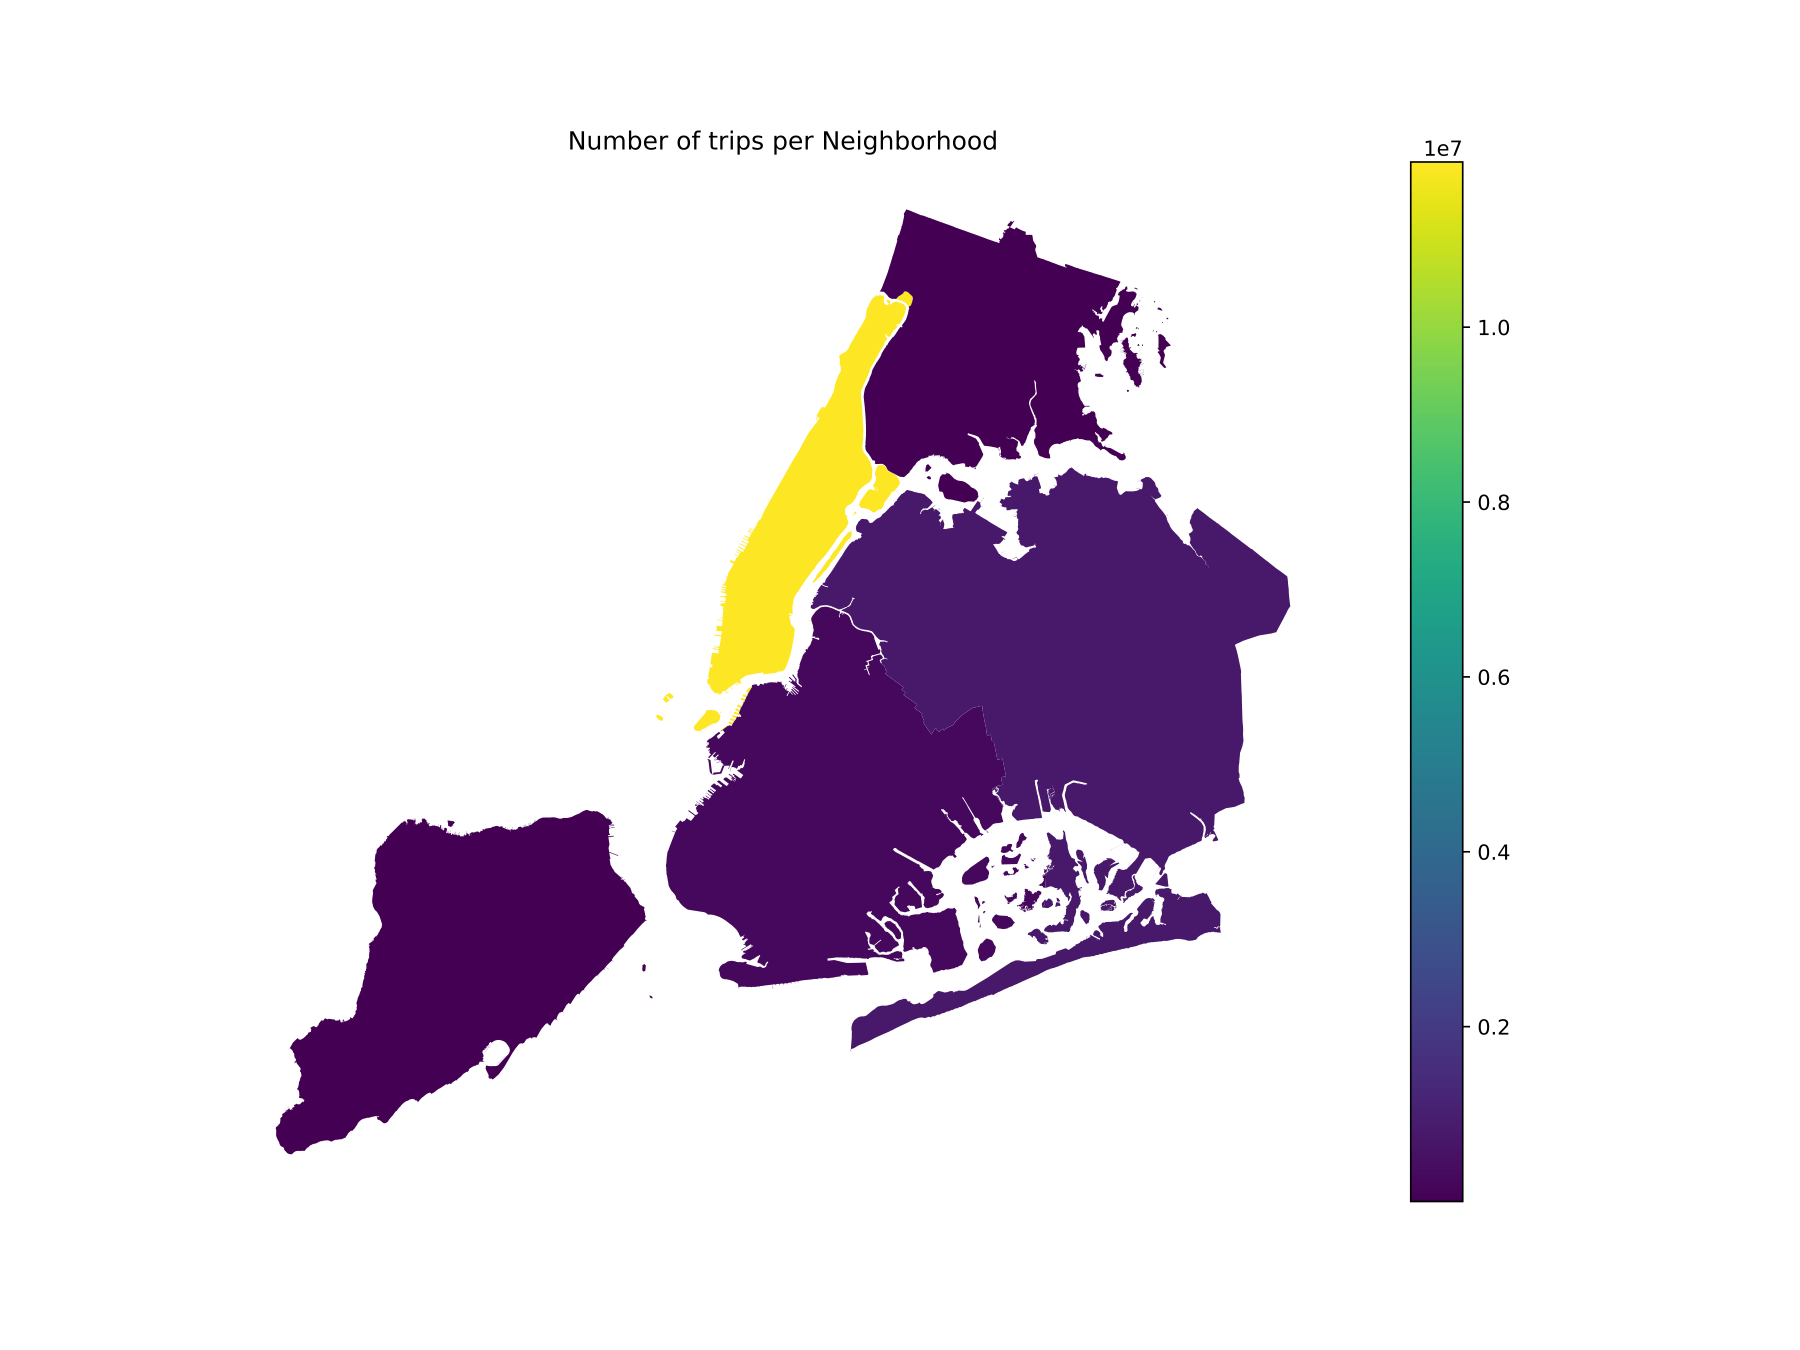
\includegraphics{figs/chloro_NY_neighborhoods.png}
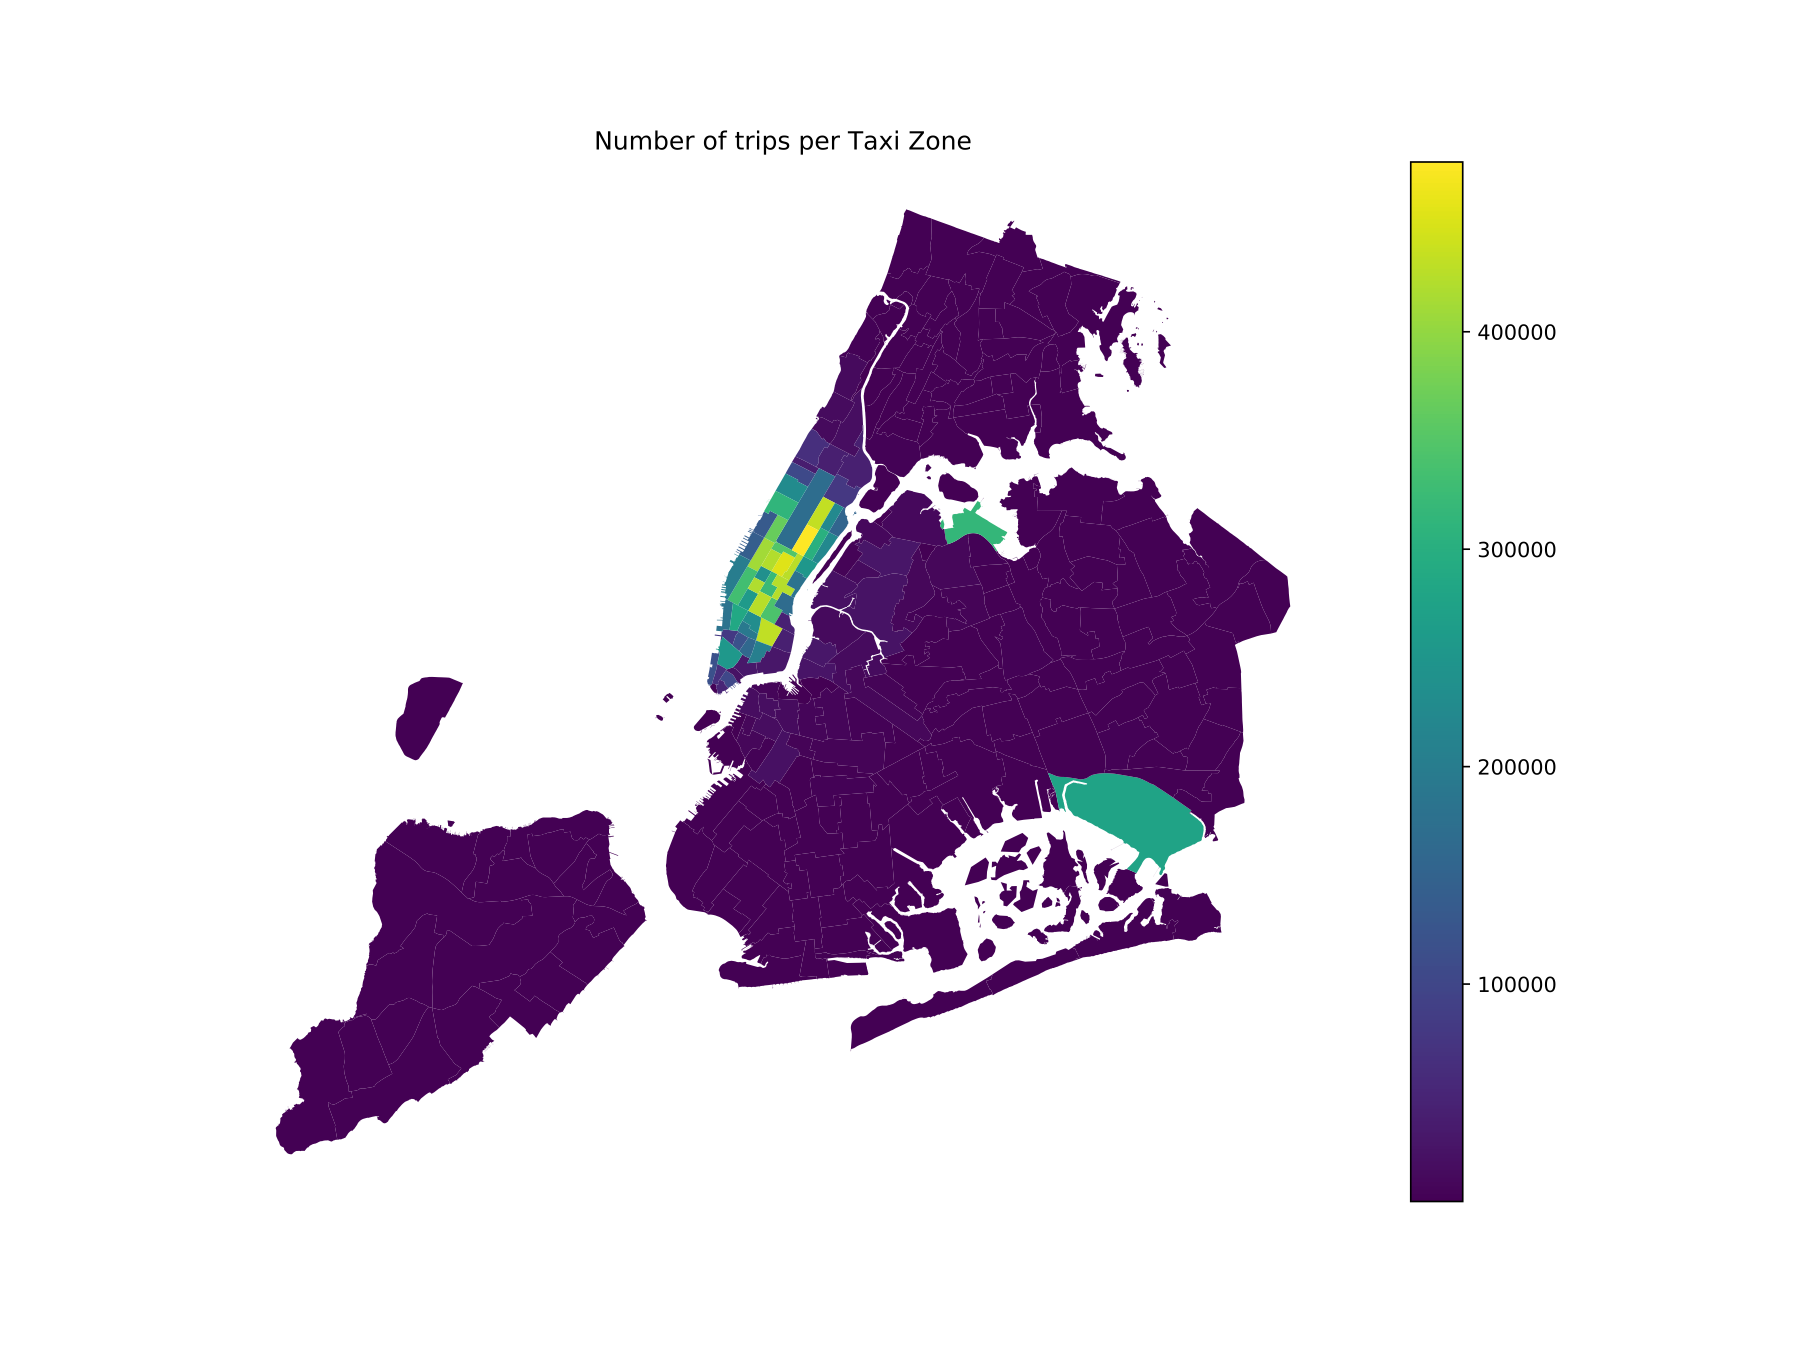
\includegraphics{figs/chloro_NY_taxi_zones.png}

    \subsection{4: Temporal features}\label{temporal-features}

We can utilize the \texttt{start\_timestamp} column to design a lot of
interesting features.

    We implement the following temporal (related to time) features using the
\texttt{add\_time\_columns} function below. - \texttt{month} derived
from \texttt{start\_timestamp}. - \texttt{week\_of\_year} derived from
\texttt{start\_timestamp}. - \texttt{day\_of\_month} derived from
\texttt{start\_timestamp}. - \texttt{day\_of\_week} derived from
\texttt{start\_timestamp}. - \texttt{hour} derived from
\texttt{start\_timestamp}. - \texttt{week\_hour} derived from
\texttt{start\_timestamp}.

\textbf{Note 1}: You can use the \texttt{dt} attribute of the
\texttt{start\_timestamp} column to convert the entry into a
\texttt{DateTime} object.

\textbf{Note 2}: We set \texttt{df.is\_copy\ =\ False} to explicitly
write back to the original dataframe, \texttt{df}, that is being passed
into the \texttt{add\_time\_columns} function. Otherwise \texttt{pandas}
will complain.

    \begin{Verbatim}[commandchars=\\\{\}]
{\color{incolor}In [{\color{incolor}17}]:} \PY{k}{def} \PY{n+nf}{add\PYZus{}time\PYZus{}columns}\PY{p}{(}\PY{n}{df}\PY{p}{)}\PY{p}{:}
             \PY{l+s+sd}{\PYZdq{}\PYZdq{}\PYZdq{}}
         \PY{l+s+sd}{    Add temporal features to df}
         \PY{l+s+sd}{    \PYZdq{}\PYZdq{}\PYZdq{}}
             \PY{n}{df}\PY{o}{.}\PY{n}{is\PYZus{}copy} \PY{o}{=} \PY{k+kc}{False} 
             \PY{n}{df}\PY{o}{.}\PY{n}{loc}\PY{p}{[}\PY{p}{:}\PY{p}{,} \PY{l+s+s1}{\PYZsq{}}\PY{l+s+s1}{month}\PY{l+s+s1}{\PYZsq{}}\PY{p}{]} \PY{o}{=} \PY{n}{df}\PY{p}{[}\PY{l+s+s1}{\PYZsq{}}\PY{l+s+s1}{tpep\PYZus{}pickup\PYZus{}datetime}\PY{l+s+s1}{\PYZsq{}}\PY{p}{]}\PY{o}{.}\PY{n}{dt}\PY{o}{.}\PY{n}{month}
             \PY{n}{df}\PY{o}{.}\PY{n}{loc}\PY{p}{[}\PY{p}{:}\PY{p}{,} \PY{l+s+s1}{\PYZsq{}}\PY{l+s+s1}{week\PYZus{}of\PYZus{}year}\PY{l+s+s1}{\PYZsq{}}\PY{p}{]} \PY{o}{=} \PY{n}{df}\PY{p}{[}\PY{l+s+s1}{\PYZsq{}}\PY{l+s+s1}{tpep\PYZus{}pickup\PYZus{}datetime}\PY{l+s+s1}{\PYZsq{}}\PY{p}{]}\PY{o}{.}\PY{n}{dt}\PY{o}{.}\PY{n}{weekofyear}
             \PY{n}{df}\PY{o}{.}\PY{n}{loc}\PY{p}{[}\PY{p}{:}\PY{p}{,} \PY{l+s+s1}{\PYZsq{}}\PY{l+s+s1}{day\PYZus{}of\PYZus{}month}\PY{l+s+s1}{\PYZsq{}}\PY{p}{]} \PY{o}{=} \PY{n}{df}\PY{p}{[}\PY{l+s+s1}{\PYZsq{}}\PY{l+s+s1}{tpep\PYZus{}pickup\PYZus{}datetime}\PY{l+s+s1}{\PYZsq{}}\PY{p}{]}\PY{o}{.}\PY{n}{dt}\PY{o}{.}\PY{n}{day}
             \PY{n}{df}\PY{o}{.}\PY{n}{loc}\PY{p}{[}\PY{p}{:}\PY{p}{,} \PY{l+s+s1}{\PYZsq{}}\PY{l+s+s1}{day\PYZus{}of\PYZus{}week}\PY{l+s+s1}{\PYZsq{}}\PY{p}{]} \PY{o}{=} \PY{n}{df}\PY{p}{[}\PY{l+s+s1}{\PYZsq{}}\PY{l+s+s1}{tpep\PYZus{}pickup\PYZus{}datetime}\PY{l+s+s1}{\PYZsq{}}\PY{p}{]}\PY{o}{.}\PY{n}{dt}\PY{o}{.}\PY{n}{dayofweek}
             \PY{n}{df}\PY{o}{.}\PY{n}{loc}\PY{p}{[}\PY{p}{:}\PY{p}{,} \PY{l+s+s1}{\PYZsq{}}\PY{l+s+s1}{hour}\PY{l+s+s1}{\PYZsq{}}\PY{p}{]} \PY{o}{=} \PY{n}{df}\PY{p}{[}\PY{l+s+s1}{\PYZsq{}}\PY{l+s+s1}{tpep\PYZus{}pickup\PYZus{}datetime}\PY{l+s+s1}{\PYZsq{}}\PY{p}{]}\PY{o}{.}\PY{n}{dt}\PY{o}{.}\PY{n}{hour}
             \PY{n}{df}\PY{o}{.}\PY{n}{loc}\PY{p}{[}\PY{p}{:}\PY{p}{,} \PY{l+s+s1}{\PYZsq{}}\PY{l+s+s1}{week\PYZus{}hour}\PY{l+s+s1}{\PYZsq{}}\PY{p}{]} \PY{o}{=} \PY{n}{df}\PY{p}{[}\PY{l+s+s1}{\PYZsq{}}\PY{l+s+s1}{tpep\PYZus{}pickup\PYZus{}datetime}\PY{l+s+s1}{\PYZsq{}}\PY{p}{]}\PY{o}{.}\PY{n}{dt}\PY{o}{.}\PY{n}{weekday} \PY{o}{*} \PY{l+m+mi}{24} \PY{o}{+} \PY{n}{df}\PY{p}{[}\PY{l+s+s1}{\PYZsq{}}\PY{l+s+s1}{hour}\PY{l+s+s1}{\PYZsq{}}\PY{p}{]}
          
             \PY{c+c1}{\PYZsh{} No real need to return here, but we harmonize with remove\PYZus{}outliers for later pipelinezation}
             \PY{k}{return} \PY{n}{df}
\end{Verbatim}


    \begin{Verbatim}[commandchars=\\\{\}]
{\color{incolor}In [{\color{incolor}18}]:} \PY{c+c1}{\PYZsh{} Note that we are applying this transformation to train\PYZus{}df, short\PYZus{}rides and long\PYZus{}rides}
         \PY{n}{train\PYZus{}df} \PY{o}{=} \PY{n}{add\PYZus{}time\PYZus{}columns}\PY{p}{(}\PY{n}{train\PYZus{}df}\PY{p}{)}
         \PY{n}{short\PYZus{}rides} \PY{o}{=} \PY{n}{add\PYZus{}time\PYZus{}columns}\PY{p}{(}\PY{n}{short\PYZus{}rides}\PY{p}{)}
         \PY{n}{long\PYZus{}rides} \PY{o}{=} \PY{n}{add\PYZus{}time\PYZus{}columns}\PY{p}{(}\PY{n}{long\PYZus{}rides}\PY{p}{)}
\end{Verbatim}


    \begin{Verbatim}[commandchars=\\\{\}]
/srv/conda/envs/data100/lib/python3.6/site-packages/pandas/core/generic.py:4388: FutureWarning: Attribute 'is\_copy' is deprecated and will be removed in a future version.
  object.\_\_getattribute\_\_(self, name)
/srv/conda/envs/data100/lib/python3.6/site-packages/pandas/core/generic.py:4389: FutureWarning: Attribute 'is\_copy' is deprecated and will be removed in a future version.
  return object.\_\_setattr\_\_(self, name, value)

    \end{Verbatim}

    \begin{Verbatim}[commandchars=\\\{\}]
{\color{incolor}In [{\color{incolor}19}]:} \PY{n}{train\PYZus{}df}\PY{p}{[}\PY{p}{[}\PY{l+s+s1}{\PYZsq{}}\PY{l+s+s1}{month}\PY{l+s+s1}{\PYZsq{}}\PY{p}{,} \PY{l+s+s1}{\PYZsq{}}\PY{l+s+s1}{week\PYZus{}of\PYZus{}year}\PY{l+s+s1}{\PYZsq{}}\PY{p}{,} \PY{l+s+s1}{\PYZsq{}}\PY{l+s+s1}{day\PYZus{}of\PYZus{}month}\PY{l+s+s1}{\PYZsq{}}\PY{p}{,} \PY{l+s+s1}{\PYZsq{}}\PY{l+s+s1}{day\PYZus{}of\PYZus{}week}\PY{l+s+s1}{\PYZsq{}}\PY{p}{,} \PY{l+s+s1}{\PYZsq{}}\PY{l+s+s1}{hour}\PY{l+s+s1}{\PYZsq{}}\PY{p}{,} \PY{l+s+s1}{\PYZsq{}}\PY{l+s+s1}{week\PYZus{}hour}\PY{l+s+s1}{\PYZsq{}}\PY{p}{]}\PY{p}{]}\PY{o}{.}\PY{n}{head}\PY{p}{(}\PY{p}{)}
\end{Verbatim}


\begin{Verbatim}[commandchars=\\\{\}]
{\color{outcolor}Out[{\color{outcolor}19}]:}        month  week\_of\_year  day\_of\_month  day\_of\_week  hour  week\_hour
         16434      1             3            21            3    17         89
         21929      1             4            29            4    23        119
         3370       1             1             5            1    18         42
         21975      1             4            30            5     0        120
         13758      1             3            18            0    13         13
\end{Verbatim}
            
    Your \texttt{train\_df.head()} should look like this, although the
ordering of the data in \texttt{id} might be different:
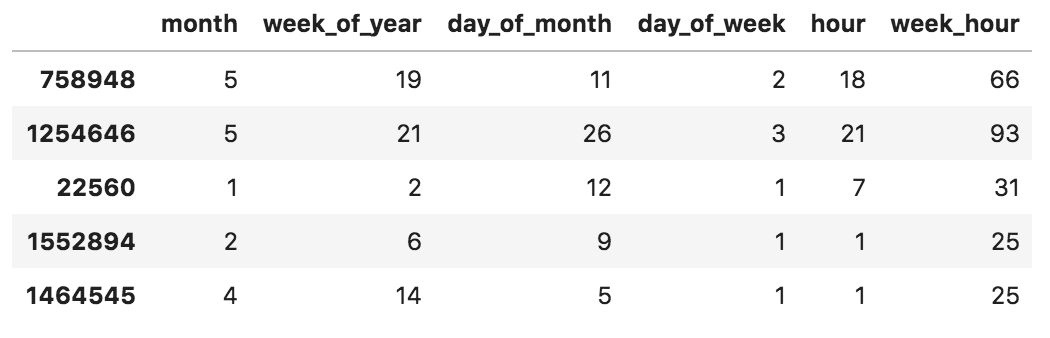
\includegraphics{figs/time_columns.png}

    \begin{Verbatim}[commandchars=\\\{\}]
{\color{incolor}In [{\color{incolor}20}]:} \PY{n}{time\PYZus{}columns} \PY{o}{=} \PY{p}{[}\PY{l+s+s1}{\PYZsq{}}\PY{l+s+s1}{month}\PY{l+s+s1}{\PYZsq{}}\PY{p}{,}
                         \PY{l+s+s1}{\PYZsq{}}\PY{l+s+s1}{week\PYZus{}of\PYZus{}year}\PY{l+s+s1}{\PYZsq{}}\PY{p}{,}
                         \PY{l+s+s1}{\PYZsq{}}\PY{l+s+s1}{day\PYZus{}of\PYZus{}month}\PY{l+s+s1}{\PYZsq{}}\PY{p}{,}
                         \PY{l+s+s1}{\PYZsq{}}\PY{l+s+s1}{day\PYZus{}of\PYZus{}week}\PY{l+s+s1}{\PYZsq{}}\PY{p}{,}
                         \PY{l+s+s1}{\PYZsq{}}\PY{l+s+s1}{hour}\PY{l+s+s1}{\PYZsq{}}\PY{p}{,}
                         \PY{l+s+s1}{\PYZsq{}}\PY{l+s+s1}{week\PYZus{}hour}\PY{l+s+s1}{\PYZsq{}}\PY{p}{]}
         
         
         \PY{c+c1}{\PYZsh{} Check columns were created}
         \PY{k}{assert} \PY{n+nb}{all}\PY{p}{(}\PY{n}{column} \PY{o+ow}{in} \PY{n}{train\PYZus{}df}\PY{o}{.}\PY{n}{columns} \PY{k}{for} \PY{n}{column} \PY{o+ow}{in} \PY{n}{time\PYZus{}columns}\PY{p}{)}
         
         \PY{c+c1}{\PYZsh{} Check type}
         \PY{k}{assert} \PY{n}{train\PYZus{}df}\PY{p}{[}\PY{n}{time\PYZus{}columns}\PY{p}{]}\PY{o}{.}\PY{n}{dtypes}\PY{o}{.}\PY{n}{nunique}\PY{p}{(}\PY{p}{)} \PY{o}{==} \PY{l+m+mi}{1}
         
         \PY{k}{assert} \PY{n}{train\PYZus{}df}\PY{p}{[}\PY{n}{time\PYZus{}columns}\PY{p}{]}\PY{o}{.}\PY{n}{dtypes}\PY{o}{.}\PY{n}{nunique}\PY{p}{(}\PY{p}{)} \PY{o}{==} \PY{l+m+mi}{1}
\end{Verbatim}


    \subsubsection{Visualizing Temporal
Features}\label{visualizing-temporal-features}

    \subsubsection{Question 4a}\label{question-4a}

Let us now use the features we created to plot some histograms and
visualize patterns in our dataset. We will analyze the distribution of
the number of taxi rides across months and days of the week. This can
help us visualize and understand patterns and trends within our data.

This is a open ended question. Create 2 plots that visualize temporal
information from our dataset. At least one of them must visualize the
hour of each day. Aside from that you can use any column from
\texttt{time\_columns}.

You can use the same column multiple times, but if the plots are
redundant you will not receive full credit. This will be graded based on
how informative each plot is and how "good" the visualization is
(remember what good/bad visualizations look like for different kinds of
data!).

    \begin{Verbatim}[commandchars=\\\{\}]
{\color{incolor}In [{\color{incolor}21}]:} \PY{n}{time\PYZus{}columns}
         \PY{c+c1}{\PYZsh{}short\PYZus{}rides[\PYZsq{}day\PYZus{}of\PYZus{}week\PYZsq{}].value\PYZus{}counts()}
\end{Verbatim}


\begin{Verbatim}[commandchars=\\\{\}]
{\color{outcolor}Out[{\color{outcolor}21}]:} ['month', 'week\_of\_year', 'day\_of\_month', 'day\_of\_week', 'hour', 'week\_hour']
\end{Verbatim}
            
    \begin{Verbatim}[commandchars=\\\{\}]
{\color{incolor}In [{\color{incolor}22}]:} \PY{c+c1}{\PYZsh{}sns.distplot(short\PYZus{}rides[\PYZsq{}day\PYZus{}of\PYZus{}week\PYZsq{}], bins = np.arange(\PYZhy{}1, 7, 1)+.5, kde = False, norm\PYZus{}hist = True)}
         \PY{c+c1}{\PYZsh{}plt.xlim(\PYZhy{}.5, 6.5)}
         \PY{c+c1}{\PYZsh{}plt.xticks(np.arange(0, 7, 1))}
         \PY{c+c1}{\PYZsh{}plt.title(\PYZsq{}Distribution of Short Ride Proportion by Day of the Week\PYZsq{})}
         \PY{c+c1}{\PYZsh{}plt.ylabel(\PYZsq{}Proportion\PYZsq{})}
\end{Verbatim}


    \paragraph{Visualization 1}\label{visualization-1}

    \begin{Verbatim}[commandchars=\\\{\}]
{\color{incolor}In [{\color{incolor}23}]:} \PY{c+c1}{\PYZsh{} Visualization 1}
         \PY{n}{plt}\PY{o}{.}\PY{n}{figure}\PY{p}{(}\PY{n}{figsize} \PY{o}{=} \PY{p}{(}\PY{l+m+mi}{15}\PY{p}{,} \PY{l+m+mi}{12}\PY{p}{)}\PY{p}{)}
         
         
         \PY{c+c1}{\PYZsh{}\PYZsh{}\PYZsh{} Plot 1}
         \PY{n}{plt}\PY{o}{.}\PY{n}{subplot}\PY{p}{(}\PY{l+m+mi}{2}\PY{p}{,}\PY{l+m+mi}{2}\PY{p}{,}\PY{l+m+mi}{1}\PY{p}{)}
         \PY{n}{sns}\PY{o}{.}\PY{n}{distplot}\PY{p}{(}\PY{n}{short\PYZus{}rides}\PY{p}{[}\PY{l+s+s1}{\PYZsq{}}\PY{l+s+s1}{hour}\PY{l+s+s1}{\PYZsq{}}\PY{p}{]}\PY{p}{,} \PY{n}{bins} \PY{o}{=} \PY{n}{np}\PY{o}{.}\PY{n}{arange}\PY{p}{(}\PY{o}{\PYZhy{}}\PY{l+m+mi}{1}\PY{p}{,} \PY{l+m+mi}{25}\PY{p}{,} \PY{l+m+mi}{1}\PY{p}{)}\PY{o}{+}\PY{o}{.}\PY{l+m+mi}{5}\PY{p}{)}
         \PY{n}{plt}\PY{o}{.}\PY{n}{xlim}\PY{p}{(}\PY{o}{\PYZhy{}}\PY{o}{.}\PY{l+m+mi}{5}\PY{p}{,} \PY{l+m+mf}{23.5}\PY{p}{)}
         \PY{n}{plt}\PY{o}{.}\PY{n}{xticks}\PY{p}{(}\PY{n}{np}\PY{o}{.}\PY{n}{arange}\PY{p}{(}\PY{l+m+mi}{0}\PY{p}{,} \PY{l+m+mi}{24}\PY{p}{,} \PY{l+m+mi}{1}\PY{p}{)}\PY{p}{)}
         \PY{n}{plt}\PY{o}{.}\PY{n}{title}\PY{p}{(}\PY{l+s+s1}{\PYZsq{}}\PY{l+s+s1}{Distribution of Short Ride Proportion by Hour}\PY{l+s+s1}{\PYZsq{}}\PY{p}{)}
         \PY{n}{plt}\PY{o}{.}\PY{n}{ylabel}\PY{p}{(}\PY{l+s+s1}{\PYZsq{}}\PY{l+s+s1}{Proportion}\PY{l+s+s1}{\PYZsq{}}\PY{p}{)}
         
         \PY{c+c1}{\PYZsh{}\PYZsh{}\PYZsh{} Plot 2}
         \PY{n}{plt}\PY{o}{.}\PY{n}{subplot}\PY{p}{(}\PY{l+m+mi}{2}\PY{p}{,}\PY{l+m+mi}{2}\PY{p}{,}\PY{l+m+mi}{3}\PY{p}{)}
         
         \PY{n}{sns}\PY{o}{.}\PY{n}{distplot}\PY{p}{(}\PY{n}{long\PYZus{}rides}\PY{p}{[}\PY{l+s+s1}{\PYZsq{}}\PY{l+s+s1}{hour}\PY{l+s+s1}{\PYZsq{}}\PY{p}{]}\PY{p}{,} \PY{n}{bins} \PY{o}{=} \PY{n}{np}\PY{o}{.}\PY{n}{arange}\PY{p}{(}\PY{o}{\PYZhy{}}\PY{l+m+mi}{1}\PY{p}{,} \PY{l+m+mi}{25}\PY{p}{,} \PY{l+m+mi}{1}\PY{p}{)}\PY{o}{+}\PY{o}{.}\PY{l+m+mi}{5}\PY{p}{)}
         \PY{n}{plt}\PY{o}{.}\PY{n}{xlim}\PY{p}{(}\PY{o}{\PYZhy{}}\PY{o}{.}\PY{l+m+mi}{5}\PY{p}{,} \PY{l+m+mf}{23.5}\PY{p}{)}
         \PY{n}{plt}\PY{o}{.}\PY{n}{xticks}\PY{p}{(}\PY{n}{np}\PY{o}{.}\PY{n}{arange}\PY{p}{(}\PY{l+m+mi}{0}\PY{p}{,} \PY{l+m+mi}{24}\PY{p}{,} \PY{l+m+mi}{1}\PY{p}{)}\PY{p}{)}
         \PY{n}{plt}\PY{o}{.}\PY{n}{title}\PY{p}{(}\PY{l+s+s1}{\PYZsq{}}\PY{l+s+s1}{Distribution of Long Ride Proportion by Hour}\PY{l+s+s1}{\PYZsq{}}\PY{p}{)}
         \PY{n}{plt}\PY{o}{.}\PY{n}{ylabel}\PY{p}{(}\PY{l+s+s1}{\PYZsq{}}\PY{l+s+s1}{Proportion}\PY{l+s+s1}{\PYZsq{}}\PY{p}{)}
         
         \PY{c+c1}{\PYZsh{}\PYZsh{}\PYZsh{} Plot 3}
         \PY{n}{plt}\PY{o}{.}\PY{n}{subplot}\PY{p}{(}\PY{l+m+mi}{2}\PY{p}{,}\PY{l+m+mi}{2}\PY{p}{,}\PY{l+m+mi}{2}\PY{p}{)}
         
         \PY{n}{sns}\PY{o}{.}\PY{n}{distplot}\PY{p}{(}\PY{n}{short\PYZus{}rides}\PY{p}{[}\PY{l+s+s1}{\PYZsq{}}\PY{l+s+s1}{hour}\PY{l+s+s1}{\PYZsq{}}\PY{p}{]}\PY{p}{,} \PY{n}{hist} \PY{o}{=} \PY{k+kc}{False}\PY{p}{,} \PY{n}{bins} \PY{o}{=} \PY{n}{np}\PY{o}{.}\PY{n}{arange}\PY{p}{(}\PY{o}{\PYZhy{}}\PY{l+m+mi}{1}\PY{p}{,} \PY{l+m+mi}{25}\PY{p}{,} \PY{l+m+mi}{1}\PY{p}{)}\PY{p}{,} \PY{n}{label} \PY{o}{=} \PY{l+s+s1}{\PYZsq{}}\PY{l+s+s1}{Short Rides}\PY{l+s+s1}{\PYZsq{}}\PY{p}{)}
         \PY{n}{plt}\PY{o}{.}\PY{n}{xlim}\PY{p}{(}\PY{l+m+mi}{0}\PY{p}{,} \PY{l+m+mi}{24}\PY{p}{)}
         \PY{n}{plt}\PY{o}{.}\PY{n}{xticks}\PY{p}{(}\PY{n}{np}\PY{o}{.}\PY{n}{arange}\PY{p}{(}\PY{l+m+mi}{0}\PY{p}{,} \PY{l+m+mi}{24}\PY{p}{,} \PY{l+m+mi}{1}\PY{p}{)}\PY{p}{)}
         \PY{n}{plt}\PY{o}{.}\PY{n}{ylabel}\PY{p}{(}\PY{l+s+s1}{\PYZsq{}}\PY{l+s+s1}{Proportion}\PY{l+s+s1}{\PYZsq{}}\PY{p}{)}
         
         \PY{n}{sns}\PY{o}{.}\PY{n}{distplot}\PY{p}{(}\PY{n}{long\PYZus{}rides}\PY{p}{[}\PY{l+s+s1}{\PYZsq{}}\PY{l+s+s1}{hour}\PY{l+s+s1}{\PYZsq{}}\PY{p}{]}\PY{p}{,} \PY{n}{hist} \PY{o}{=} \PY{k+kc}{False}\PY{p}{,} \PY{n}{bins} \PY{o}{=} \PY{n}{np}\PY{o}{.}\PY{n}{arange}\PY{p}{(}\PY{o}{\PYZhy{}}\PY{l+m+mi}{1}\PY{p}{,} \PY{l+m+mi}{25}\PY{p}{,} \PY{l+m+mi}{1}\PY{p}{)}\PY{p}{,} \PY{n}{label} \PY{o}{=} \PY{l+s+s1}{\PYZsq{}}\PY{l+s+s1}{Long Rides}\PY{l+s+s1}{\PYZsq{}}\PY{p}{)}
         \PY{n}{plt}\PY{o}{.}\PY{n}{xlim}\PY{p}{(}\PY{l+m+mi}{0}\PY{p}{,} \PY{l+m+mi}{24}\PY{p}{)}
         \PY{n}{plt}\PY{o}{.}\PY{n}{legend}\PY{p}{(}\PY{p}{)}
         \PY{n}{plt}\PY{o}{.}\PY{n}{xticks}\PY{p}{(}\PY{n}{np}\PY{o}{.}\PY{n}{arange}\PY{p}{(}\PY{l+m+mi}{0}\PY{p}{,} \PY{l+m+mi}{24}\PY{p}{,} \PY{l+m+mi}{1}\PY{p}{)}\PY{p}{)}
         \PY{n}{plt}\PY{o}{.}\PY{n}{ylabel}\PY{p}{(}\PY{l+s+s1}{\PYZsq{}}\PY{l+s+s1}{Proportion}\PY{l+s+s1}{\PYZsq{}}\PY{p}{)}
         
         \PY{n}{plt}\PY{o}{.}\PY{n}{title}\PY{p}{(}\PY{l+s+s1}{\PYZsq{}}\PY{l+s+s1}{Superimposed KDEs of Ride Proportions by Hour}\PY{l+s+s1}{\PYZsq{}}\PY{p}{)}
         
         \PY{c+c1}{\PYZsh{}\PYZsh{}\PYZsh{} Plot 4}
         \PY{n}{plt}\PY{o}{.}\PY{n}{subplot}\PY{p}{(}\PY{l+m+mi}{2}\PY{p}{,}\PY{l+m+mi}{2}\PY{p}{,}\PY{l+m+mi}{4}\PY{p}{)}
         
         \PY{n}{sns}\PY{o}{.}\PY{n}{distplot}\PY{p}{(}\PY{n}{short\PYZus{}rides}\PY{p}{[}\PY{l+s+s1}{\PYZsq{}}\PY{l+s+s1}{hour}\PY{l+s+s1}{\PYZsq{}}\PY{p}{]}\PY{p}{,} \PY{n}{kde} \PY{o}{=} \PY{k+kc}{False}\PY{p}{,} \PY{n}{norm\PYZus{}hist} \PY{o}{=} \PY{k+kc}{True}\PY{p}{,} \PY{n}{bins} \PY{o}{=} \PY{n}{np}\PY{o}{.}\PY{n}{arange}\PY{p}{(}\PY{o}{\PYZhy{}}\PY{l+m+mi}{1}\PY{p}{,} \PY{l+m+mi}{25}\PY{p}{,} \PY{l+m+mi}{1}\PY{p}{)}\PY{o}{+}\PY{o}{.}\PY{l+m+mi}{5}\PY{p}{,} \PY{n}{label} \PY{o}{=} \PY{l+s+s1}{\PYZsq{}}\PY{l+s+s1}{Short Rides}\PY{l+s+s1}{\PYZsq{}}\PY{p}{)}
         \PY{n}{plt}\PY{o}{.}\PY{n}{xlim}\PY{p}{(}\PY{o}{\PYZhy{}}\PY{o}{.}\PY{l+m+mi}{5}\PY{p}{,} \PY{l+m+mf}{23.5}\PY{p}{)}
         \PY{n}{plt}\PY{o}{.}\PY{n}{xticks}\PY{p}{(}\PY{n}{np}\PY{o}{.}\PY{n}{arange}\PY{p}{(}\PY{l+m+mi}{0}\PY{p}{,} \PY{l+m+mi}{24}\PY{p}{,} \PY{l+m+mi}{1}\PY{p}{)}\PY{p}{)}
         \PY{n}{plt}\PY{o}{.}\PY{n}{ylabel}\PY{p}{(}\PY{l+s+s1}{\PYZsq{}}\PY{l+s+s1}{Proportion}\PY{l+s+s1}{\PYZsq{}}\PY{p}{)}
         
         \PY{n}{sns}\PY{o}{.}\PY{n}{distplot}\PY{p}{(}\PY{n}{long\PYZus{}rides}\PY{p}{[}\PY{l+s+s1}{\PYZsq{}}\PY{l+s+s1}{hour}\PY{l+s+s1}{\PYZsq{}}\PY{p}{]}\PY{p}{,} \PY{n}{kde} \PY{o}{=} \PY{k+kc}{False}\PY{p}{,} \PY{n}{norm\PYZus{}hist} \PY{o}{=} \PY{k+kc}{True}\PY{p}{,} \PY{n}{bins} \PY{o}{=} \PY{n}{np}\PY{o}{.}\PY{n}{arange}\PY{p}{(}\PY{o}{\PYZhy{}}\PY{l+m+mi}{1}\PY{p}{,} \PY{l+m+mi}{25}\PY{p}{,} \PY{l+m+mi}{1}\PY{p}{)}\PY{o}{+}\PY{o}{.}\PY{l+m+mi}{5}\PY{p}{,} \PY{n}{label} \PY{o}{=} \PY{l+s+s1}{\PYZsq{}}\PY{l+s+s1}{Long Rides}\PY{l+s+s1}{\PYZsq{}}\PY{p}{)}
         \PY{n}{plt}\PY{o}{.}\PY{n}{xlim}\PY{p}{(}\PY{o}{\PYZhy{}}\PY{o}{.}\PY{l+m+mi}{5}\PY{p}{,} \PY{l+m+mf}{23.5}\PY{p}{)}
         \PY{n}{plt}\PY{o}{.}\PY{n}{xticks}\PY{p}{(}\PY{n}{np}\PY{o}{.}\PY{n}{arange}\PY{p}{(}\PY{l+m+mi}{0}\PY{p}{,} \PY{l+m+mi}{24}\PY{p}{,} \PY{l+m+mi}{1}\PY{p}{)}\PY{p}{)}
         \PY{n}{plt}\PY{o}{.}\PY{n}{ylabel}\PY{p}{(}\PY{l+s+s1}{\PYZsq{}}\PY{l+s+s1}{Proportion}\PY{l+s+s1}{\PYZsq{}}\PY{p}{)}
         \PY{n}{plt}\PY{o}{.}\PY{n}{title}\PY{p}{(}\PY{l+s+s1}{\PYZsq{}}\PY{l+s+s1}{Superimposed Distribution of Ride Proportions by Hour}\PY{l+s+s1}{\PYZsq{}}\PY{p}{)}
         \PY{n}{plt}\PY{o}{.}\PY{n}{legend}\PY{p}{(}\PY{p}{)}
         
         \PY{n}{plt}\PY{o}{.}\PY{n}{suptitle}\PY{p}{(}\PY{l+s+s1}{\PYZsq{}}\PY{l+s+s1}{Proportion of Rides per Hour of the Day.}\PY{l+s+s1}{\PYZsq{}}\PY{p}{)}
         
         \PY{n}{plt}\PY{o}{.}\PY{n}{show}\PY{p}{(}\PY{p}{)}
\end{Verbatim}


    \begin{center}
    \adjustimage{max size={0.9\linewidth}{0.9\paperheight}}{output_48_0.png}
    \end{center}
    { \hspace*{\fill} \\}
    
    \paragraph{Visualization 2}\label{visualization-2}

    \begin{Verbatim}[commandchars=\\\{\}]
{\color{incolor}In [{\color{incolor}24}]:} \PY{c+c1}{\PYZsh{} Visualization 2}
         
         \PY{c+c1}{\PYZsh{} Monday = 0, Sunday = 6}
         
         \PY{n}{days\PYZus{}of\PYZus{}week} \PY{o}{=} \PY{p}{[}\PY{l+s+s2}{\PYZdq{}}\PY{l+s+s2}{Mon}\PY{l+s+s2}{\PYZdq{}}\PY{p}{,} \PY{l+s+s2}{\PYZdq{}}\PY{l+s+s2}{Tue}\PY{l+s+s2}{\PYZdq{}}\PY{p}{,} \PY{l+s+s2}{\PYZdq{}}\PY{l+s+s2}{Wed}\PY{l+s+s2}{\PYZdq{}}\PY{p}{,} \PY{l+s+s2}{\PYZdq{}}\PY{l+s+s2}{Thu}\PY{l+s+s2}{\PYZdq{}}\PY{p}{,} \PY{l+s+s2}{\PYZdq{}}\PY{l+s+s2}{Fri}\PY{l+s+s2}{\PYZdq{}}\PY{p}{,} \PY{l+s+s2}{\PYZdq{}}\PY{l+s+s2}{Sat}\PY{l+s+s2}{\PYZdq{}}\PY{p}{,} \PY{l+s+s2}{\PYZdq{}}\PY{l+s+s2}{Sun}\PY{l+s+s2}{\PYZdq{}}\PY{p}{]}
         
         \PY{n}{plt}\PY{o}{.}\PY{n}{figure}\PY{p}{(}\PY{n}{figsize} \PY{o}{=} \PY{p}{(}\PY{l+m+mi}{15}\PY{p}{,} \PY{l+m+mi}{12}\PY{p}{)}\PY{p}{)}
         
         
         \PY{c+c1}{\PYZsh{}\PYZsh{}\PYZsh{} Plot 1}
         \PY{n}{plt}\PY{o}{.}\PY{n}{subplot}\PY{p}{(}\PY{l+m+mi}{2}\PY{p}{,}\PY{l+m+mi}{2}\PY{p}{,}\PY{l+m+mi}{1}\PY{p}{)}
         
         \PY{n}{sns}\PY{o}{.}\PY{n}{distplot}\PY{p}{(}\PY{n}{short\PYZus{}rides}\PY{p}{[}\PY{l+s+s1}{\PYZsq{}}\PY{l+s+s1}{day\PYZus{}of\PYZus{}week}\PY{l+s+s1}{\PYZsq{}}\PY{p}{]}\PY{p}{,} \PY{n}{bins} \PY{o}{=} \PY{n}{np}\PY{o}{.}\PY{n}{arange}\PY{p}{(}\PY{o}{\PYZhy{}}\PY{l+m+mi}{1}\PY{p}{,} \PY{l+m+mi}{7}\PY{p}{,} \PY{l+m+mi}{1}\PY{p}{)}\PY{o}{+}\PY{o}{.}\PY{l+m+mi}{5}\PY{p}{,} \PY{n}{kde} \PY{o}{=} \PY{k+kc}{False}\PY{p}{,} \PY{n}{norm\PYZus{}hist} \PY{o}{=} \PY{k+kc}{True}\PY{p}{)}
         \PY{n}{plt}\PY{o}{.}\PY{n}{xlim}\PY{p}{(}\PY{o}{\PYZhy{}}\PY{o}{.}\PY{l+m+mi}{5}\PY{p}{,} \PY{l+m+mf}{6.5}\PY{p}{)}
         \PY{n}{plt}\PY{o}{.}\PY{n}{title}\PY{p}{(}\PY{l+s+s1}{\PYZsq{}}\PY{l+s+s1}{Distribution of Short Ride Proportion by Day of the Week}\PY{l+s+s1}{\PYZsq{}}\PY{p}{)}
         \PY{n}{plt}\PY{o}{.}\PY{n}{xticks}\PY{p}{(}\PY{p}{[}\PY{l+m+mi}{0}\PY{p}{,} \PY{l+m+mi}{1}\PY{p}{,} \PY{l+m+mi}{2}\PY{p}{,} \PY{l+m+mi}{3}\PY{p}{,} \PY{l+m+mi}{4}\PY{p}{,} \PY{l+m+mi}{5}\PY{p}{,} \PY{l+m+mi}{6}\PY{p}{]}\PY{p}{,} \PY{n}{days\PYZus{}of\PYZus{}week}\PY{p}{)}
         \PY{n}{plt}\PY{o}{.}\PY{n}{xlabel}\PY{p}{(}\PY{l+s+s1}{\PYZsq{}}\PY{l+s+s1}{\PYZsq{}}\PY{p}{)}
         \PY{n}{plt}\PY{o}{.}\PY{n}{ylabel}\PY{p}{(}\PY{l+s+s1}{\PYZsq{}}\PY{l+s+s1}{Proportion}\PY{l+s+s1}{\PYZsq{}}\PY{p}{)}
         
         \PY{c+c1}{\PYZsh{}\PYZsh{}\PYZsh{} Plot 2}
         \PY{n}{plt}\PY{o}{.}\PY{n}{subplot}\PY{p}{(}\PY{l+m+mi}{2}\PY{p}{,}\PY{l+m+mi}{2}\PY{p}{,}\PY{l+m+mi}{2}\PY{p}{)}
         
         \PY{n}{sns}\PY{o}{.}\PY{n}{distplot}\PY{p}{(}\PY{n}{long\PYZus{}rides}\PY{p}{[}\PY{l+s+s1}{\PYZsq{}}\PY{l+s+s1}{day\PYZus{}of\PYZus{}week}\PY{l+s+s1}{\PYZsq{}}\PY{p}{]}\PY{p}{,} \PY{n}{bins} \PY{o}{=} \PY{n}{np}\PY{o}{.}\PY{n}{arange}\PY{p}{(}\PY{o}{\PYZhy{}}\PY{l+m+mi}{1}\PY{p}{,} \PY{l+m+mi}{7}\PY{p}{,} \PY{l+m+mi}{1}\PY{p}{)}\PY{o}{+}\PY{o}{.}\PY{l+m+mi}{5}\PY{p}{,} \PY{n}{kde} \PY{o}{=} \PY{k+kc}{False}\PY{p}{,} \PY{n}{norm\PYZus{}hist} \PY{o}{=} \PY{k+kc}{True}\PY{p}{)}
         \PY{n}{plt}\PY{o}{.}\PY{n}{xlim}\PY{p}{(}\PY{o}{\PYZhy{}}\PY{o}{.}\PY{l+m+mi}{5}\PY{p}{,} \PY{l+m+mf}{6.5}\PY{p}{)}
         \PY{n}{plt}\PY{o}{.}\PY{n}{xticks}\PY{p}{(}\PY{p}{[}\PY{l+m+mi}{0}\PY{p}{,} \PY{l+m+mi}{1}\PY{p}{,} \PY{l+m+mi}{2}\PY{p}{,} \PY{l+m+mi}{3}\PY{p}{,} \PY{l+m+mi}{4}\PY{p}{,} \PY{l+m+mi}{5}\PY{p}{,} \PY{l+m+mi}{6}\PY{p}{]}\PY{p}{,} \PY{n}{days\PYZus{}of\PYZus{}week}\PY{p}{)}
         \PY{n}{plt}\PY{o}{.}\PY{n}{xlabel}\PY{p}{(}\PY{l+s+s1}{\PYZsq{}}\PY{l+s+s1}{\PYZsq{}}\PY{p}{)}
         \PY{n}{plt}\PY{o}{.}\PY{n}{title}\PY{p}{(}\PY{l+s+s1}{\PYZsq{}}\PY{l+s+s1}{Distribution of Long Ride Proportion by Day of the Week}\PY{l+s+s1}{\PYZsq{}}\PY{p}{)}
         \PY{n}{plt}\PY{o}{.}\PY{n}{ylabel}\PY{p}{(}\PY{l+s+s1}{\PYZsq{}}\PY{l+s+s1}{Proportion}\PY{l+s+s1}{\PYZsq{}}\PY{p}{)}
         
         
         
         \PY{c+c1}{\PYZsh{}\PYZsh{}\PYZsh{} Plot 3}
         \PY{n}{plt}\PY{o}{.}\PY{n}{subplot}\PY{p}{(}\PY{l+m+mi}{2}\PY{p}{,}\PY{l+m+mi}{2}\PY{p}{,}\PY{l+m+mi}{3}\PY{p}{)}
         
         \PY{n}{sns}\PY{o}{.}\PY{n}{distplot}\PY{p}{(}\PY{n}{short\PYZus{}rides}\PY{p}{[}\PY{l+s+s1}{\PYZsq{}}\PY{l+s+s1}{day\PYZus{}of\PYZus{}week}\PY{l+s+s1}{\PYZsq{}}\PY{p}{]}\PY{p}{,} \PY{n}{bins} \PY{o}{=} \PY{n}{np}\PY{o}{.}\PY{n}{arange}\PY{p}{(}\PY{o}{\PYZhy{}}\PY{l+m+mi}{1}\PY{p}{,} \PY{l+m+mi}{7}\PY{p}{,} \PY{l+m+mi}{1}\PY{p}{)}\PY{o}{+}\PY{o}{.}\PY{l+m+mi}{5}\PY{p}{,} \PY{n}{kde} \PY{o}{=} \PY{k+kc}{False}\PY{p}{,} \PY{n}{norm\PYZus{}hist} \PY{o}{=} \PY{k+kc}{True}\PY{p}{,} \PY{n}{label} \PY{o}{=} \PY{l+s+s1}{\PYZsq{}}\PY{l+s+s1}{Short Rides}\PY{l+s+s1}{\PYZsq{}}\PY{p}{)}
         \PY{n}{sns}\PY{o}{.}\PY{n}{distplot}\PY{p}{(}\PY{n}{long\PYZus{}rides}\PY{p}{[}\PY{l+s+s1}{\PYZsq{}}\PY{l+s+s1}{day\PYZus{}of\PYZus{}week}\PY{l+s+s1}{\PYZsq{}}\PY{p}{]}\PY{p}{,} \PY{n}{bins} \PY{o}{=} \PY{n}{np}\PY{o}{.}\PY{n}{arange}\PY{p}{(}\PY{o}{\PYZhy{}}\PY{l+m+mi}{1}\PY{p}{,} \PY{l+m+mi}{7}\PY{p}{,} \PY{l+m+mi}{1}\PY{p}{)}\PY{o}{+}\PY{o}{.}\PY{l+m+mi}{5}\PY{p}{,} \PY{n}{kde} \PY{o}{=} \PY{k+kc}{False}\PY{p}{,} \PY{n}{norm\PYZus{}hist} \PY{o}{=} \PY{k+kc}{True}\PY{p}{,} \PY{n}{label} \PY{o}{=} \PY{l+s+s1}{\PYZsq{}}\PY{l+s+s1}{Long Rides}\PY{l+s+s1}{\PYZsq{}}\PY{p}{)}
         \PY{n}{plt}\PY{o}{.}\PY{n}{xlim}\PY{p}{(}\PY{o}{\PYZhy{}}\PY{o}{.}\PY{l+m+mi}{5}\PY{p}{,} \PY{l+m+mf}{6.5}\PY{p}{)}
         \PY{n}{plt}\PY{o}{.}\PY{n}{xticks}\PY{p}{(}\PY{p}{[}\PY{l+m+mi}{0}\PY{p}{,} \PY{l+m+mi}{1}\PY{p}{,} \PY{l+m+mi}{2}\PY{p}{,} \PY{l+m+mi}{3}\PY{p}{,} \PY{l+m+mi}{4}\PY{p}{,} \PY{l+m+mi}{5}\PY{p}{,} \PY{l+m+mi}{6}\PY{p}{]}\PY{p}{,} \PY{n}{days\PYZus{}of\PYZus{}week}\PY{p}{)}
         \PY{n}{plt}\PY{o}{.}\PY{n}{xlabel}\PY{p}{(}\PY{l+s+s1}{\PYZsq{}}\PY{l+s+s1}{\PYZsq{}}\PY{p}{)}
         \PY{n}{plt}\PY{o}{.}\PY{n}{title}\PY{p}{(}\PY{l+s+s1}{\PYZsq{}}\PY{l+s+s1}{Superimposed Distribution of Short and Long Ride Proportion by Day of the Week}\PY{l+s+s1}{\PYZsq{}}\PY{p}{)}
         \PY{n}{plt}\PY{o}{.}\PY{n}{ylabel}\PY{p}{(}\PY{l+s+s1}{\PYZsq{}}\PY{l+s+s1}{Proportion}\PY{l+s+s1}{\PYZsq{}}\PY{p}{)}
         
         \PY{n}{plt}\PY{o}{.}\PY{n}{legend}\PY{p}{(}\PY{p}{)}
         
         \PY{n}{plt}\PY{o}{.}\PY{n}{suptitle}\PY{p}{(}\PY{l+s+s1}{\PYZsq{}}\PY{l+s+s1}{Proportion of Rides per Day of the Week.}\PY{l+s+s1}{\PYZsq{}}\PY{p}{)}
         
         \PY{n}{plt}\PY{o}{.}\PY{n}{show}\PY{p}{(}\PY{p}{)}
\end{Verbatim}


    \begin{center}
    \adjustimage{max size={0.9\linewidth}{0.9\paperheight}}{output_50_0.png}
    \end{center}
    { \hspace*{\fill} \\}
    
    \subsubsection{Question 4b}\label{question-4b}

Briefly explain for each plot 1. What feature you're visualization 2.
Why you chose this feature 3. Why you chose this visualization method

    \begin{Verbatim}[commandchars=\\\{\}]
{\color{incolor}In [{\color{incolor}25}]:} \PY{n}{q4b\PYZus{}answer} \PY{o}{=} \PY{l+s+sa}{r}\PY{l+s+s2}{\PYZdq{}\PYZdq{}\PYZdq{}}
         
         \PY{l+s+s2}{Visualization 1:}
         \PY{l+s+s2}{1) Plotted the histograms of proportion of rides by hour. }
         \PY{l+s+s2}{2) I chose this to get a better understanding of what time of day sees the most rides in both short and long trips,}
         \PY{l+s+s2}{and to see if there were any visible differences which might make }\PY{l+s+s2}{\PYZsq{}}\PY{l+s+s2}{hour}\PY{l+s+s2}{\PYZsq{}}\PY{l+s+s2}{ a good feature to indicate if a trip is }
         \PY{l+s+s2}{going to be long or short.}
         \PY{l+s+s2}{3) I chose a histogram since I was visualizing the count of a continuous variable. Histograms provide a good way of}
         \PY{l+s+s2}{visualizing the different proportions of each value (in this case each hour) that is easy to understand right away.}
         
         
         \PY{l+s+s2}{Visualization 2:}
         \PY{l+s+s2}{1) Plotted the histograms of proportion of rides by day of the week. }
         \PY{l+s+s2}{2) I chose this to get a better understanding of what day sees the most rides in both short and long trips,}
         \PY{l+s+s2}{and to see if there were any visible differences which might make }\PY{l+s+s2}{\PYZsq{}}\PY{l+s+s2}{day\PYZus{}of\PYZus{}week}\PY{l+s+s2}{\PYZsq{}}\PY{l+s+s2}{ a good feature to indicate if a }
         \PY{l+s+s2}{trip is going to be long or short.}
         \PY{l+s+s2}{3) I chose a histogram since I was visualizing the count of a continuous variable. Histograms provide a good way of}
         \PY{l+s+s2}{visualizing the different proportions of each value (in this case each day) that is easy to understand right away. }
         
         \PY{l+s+s2}{\PYZdq{}\PYZdq{}\PYZdq{}}
         
         
         \PY{n+nb}{print}\PY{p}{(}\PY{n}{q4b\PYZus{}answer}\PY{p}{)}
\end{Verbatim}


    \begin{Verbatim}[commandchars=\\\{\}]


Visualization 1:
1) Plotted the histograms of proportion of rides by hour. 
2) I chose this to get a better understanding of what time of day sees the most rides in both short and long trips,
and to see if there were any visible differences which might make 'hour' a good feature to indicate if a trip is 
going to be long or short.
3) I chose a histogram since I was visualizing the count of a continuous variable. Histograms provide a good way of
visualizing the different proportions of each value (in this case each hour) that is easy to understand right away.


Visualization 2:
1) Plotted the histograms of proportion of rides by day of the week. 
2) I chose this to get a better understanding of what day sees the most rides in both short and long trips,
and to see if there were any visible differences which might make 'day\_of\_week' a good feature to indicate if a 
trip is going to be long or short.
3) I chose a histogram since I was visualizing the count of a continuous variable. Histograms provide a good way of
visualizing the different proportions of each value (in this case each day) that is easy to understand right away. 



    \end{Verbatim}

    \subsubsection{Question 4c}\label{question-4c}

From the various plots above, what conclusions can you draw about the
temporal aspects of our data? How does this relate to duration?

    \begin{Verbatim}[commandchars=\\\{\}]
{\color{incolor}In [{\color{incolor}26}]:} \PY{n}{q4c\PYZus{}answer} \PY{o}{=} \PY{l+s+sa}{r}\PY{l+s+s2}{\PYZdq{}\PYZdq{}\PYZdq{}}
         \PY{l+s+s2}{From Visualization 1:}
         \PY{l+s+s2}{    in both short and long rides, the number of rides is at a low around 4\PYZhy{}5 am, increases pretty sharply from 7\PYZhy{}9am,}
         \PY{l+s+s2}{    then increases fairly steadily until global peaks at 7pm in short rides and 6pm in long rides.}
         \PY{l+s+s2}{    There are small dips in short rides at 11 am and 4pm, and a small dip in long rides around 4 pm.}
         \PY{l+s+s2}{    Purely from inspecting the superimposed graphs, we see that rides in the early hours from around 7pm to 7am have }
         \PY{l+s+s2}{    a slight tendency to be short rides, while rides from 8am until 7pm have a slight tendency to be longer rides}
         
         \PY{l+s+s2}{From Visualization 2:}
         \PY{l+s+s2}{    In short rides, we see the minimum on Mondays,  global max on Fridays with a second, shallow peak on Wednesdays. }
         \PY{l+s+s2}{    In long rides, the minimum is also Mondays and global max also Friday, but there is more of a linear buildup of }
         \PY{l+s+s2}{    rides until the max, with a sharper drop\PYZhy{}off on Saturday.}
         \PY{l+s+s2}{    The superimposed graph shows that rides on Mondays have a small tendency to be shorter rides, and rides on }
         \PY{l+s+s2}{    Saturdays and Sundays have a more significant tendency to be shorter rides. Rides on Tuesdays have a small }
         \PY{l+s+s2}{    tendency to be longer, with rides on Wednesdays and Thursdays having a more significant tendency to be longer. }
         \PY{l+s+s2}{    Fridays have a very small tendency towards longer rides}
         
         \PY{l+s+s2}{\PYZdq{}\PYZdq{}\PYZdq{}}
         
         
         \PY{n+nb}{print}\PY{p}{(}\PY{n}{q4c\PYZus{}answer}\PY{p}{)}
\end{Verbatim}


    \begin{Verbatim}[commandchars=\\\{\}]

From Visualization 1:
    in both short and long rides, the number of rides is at a low around 4-5 am, increases pretty sharply from 7-9am,
    then increases fairly steadily until global peaks at 7pm in short rides and 6pm in long rides.
    There are small dips in short rides at 11 am and 4pm, and a small dip in long rides around 4 pm.
    Purely from inspecting the superimposed graphs, we see that rides in the early hours from around 7pm to 7am have 
    a slight tendency to be short rides, while rides from 8am until 7pm have a slight tendency to be longer rides

From Visualization 2:
    In short rides, we see the minimum on Mondays,  global max on Fridays with a second, shallow peak on Wednesdays. 
    In long rides, the minimum is also Mondays and global max also Friday, but there is more of a linear buildup of 
    rides until the max, with a sharper drop-off on Saturday.
    The superimposed graph shows that rides on Mondays have a small tendency to be shorter rides, and rides on 
    Saturdays and Sundays have a more significant tendency to be shorter rides. Rides on Tuesdays have a small 
    tendency to be longer, with rides on Wednesdays and Thursdays having a more significant tendency to be longer. 
    Fridays have a very small tendency towards longer rides



    \end{Verbatim}

    \subsubsection{Question 4d}\label{question-4d}

    Previously, we have analyzed the temporal features \texttt{hour} and
\texttt{day\_of\_week} independently, but these features may in fact
have a relationship between each other. Determining the extent to their
relationship may be useful in helping us create new features in our
model. Create a violin plot that displays distribution of rides over
each hour per day of the week.

    \begin{Verbatim}[commandchars=\\\{\}]
{\color{incolor}In [{\color{incolor}27}]:} \PY{n}{fig}\PY{p}{,} \PY{n}{axes} \PY{o}{=} \PY{n}{plt}\PY{o}{.}\PY{n}{subplots}\PY{p}{(}\PY{l+m+mi}{1}\PY{p}{,} \PY{l+m+mi}{2}\PY{p}{,} \PY{n}{figsize}\PY{o}{=}\PY{p}{(}\PY{l+m+mi}{13}\PY{p}{,} \PY{l+m+mi}{4}\PY{p}{)}\PY{p}{)}
         
         \PY{n}{plt}\PY{o}{.}\PY{n}{subplot}\PY{p}{(}\PY{l+m+mi}{1}\PY{p}{,} \PY{l+m+mi}{2}\PY{p}{,} \PY{l+m+mi}{1}\PY{p}{)}
         \PY{n}{sns}\PY{o}{.}\PY{n}{violinplot}\PY{p}{(}\PY{n}{x}\PY{o}{=}\PY{l+s+s2}{\PYZdq{}}\PY{l+s+s2}{day\PYZus{}of\PYZus{}week}\PY{l+s+s2}{\PYZdq{}}\PY{p}{,} \PY{n}{y}\PY{o}{=}\PY{l+s+s2}{\PYZdq{}}\PY{l+s+s2}{hour}\PY{l+s+s2}{\PYZdq{}}\PY{p}{,} \PY{n}{data}\PY{o}{=} \PY{n}{short\PYZus{}rides}\PY{p}{)}
         \PY{n}{plt}\PY{o}{.}\PY{n}{title}\PY{p}{(}\PY{l+s+s1}{\PYZsq{}}\PY{l+s+s1}{Violin Plot of Proportion of Short Rides by Hour and Day}\PY{l+s+s1}{\PYZsq{}}\PY{p}{)}
         \PY{n}{plt}\PY{o}{.}\PY{n}{xticks}\PY{p}{(}\PY{p}{[}\PY{l+m+mi}{0}\PY{p}{,} \PY{l+m+mi}{1}\PY{p}{,} \PY{l+m+mi}{2}\PY{p}{,} \PY{l+m+mi}{3}\PY{p}{,} \PY{l+m+mi}{4}\PY{p}{,} \PY{l+m+mi}{5}\PY{p}{,} \PY{l+m+mi}{6}\PY{p}{]}\PY{p}{,} \PY{n}{days\PYZus{}of\PYZus{}week}\PY{p}{)}
         \PY{n}{plt}\PY{o}{.}\PY{n}{xlabel}\PY{p}{(}\PY{l+s+s1}{\PYZsq{}}\PY{l+s+s1}{\PYZsq{}}\PY{p}{)}
         \PY{n}{plt}\PY{o}{.}\PY{n}{ylabel}\PY{p}{(}\PY{l+s+s1}{\PYZsq{}}\PY{l+s+s1}{Hour}\PY{l+s+s1}{\PYZsq{}}\PY{p}{)}
         
         
         \PY{n}{plt}\PY{o}{.}\PY{n}{subplot}\PY{p}{(}\PY{l+m+mi}{1}\PY{p}{,} \PY{l+m+mi}{2}\PY{p}{,} \PY{l+m+mi}{2}\PY{p}{)}
         \PY{n}{sns}\PY{o}{.}\PY{n}{violinplot}\PY{p}{(}\PY{n}{x}\PY{o}{=}\PY{l+s+s2}{\PYZdq{}}\PY{l+s+s2}{day\PYZus{}of\PYZus{}week}\PY{l+s+s2}{\PYZdq{}}\PY{p}{,} \PY{n}{y}\PY{o}{=}\PY{l+s+s2}{\PYZdq{}}\PY{l+s+s2}{hour}\PY{l+s+s2}{\PYZdq{}}\PY{p}{,} \PY{n}{data}\PY{o}{=} \PY{n}{long\PYZus{}rides}\PY{p}{)}
         \PY{n}{plt}\PY{o}{.}\PY{n}{title}\PY{p}{(}\PY{l+s+s1}{\PYZsq{}}\PY{l+s+s1}{Violin Plot of Proportion of Long Rides by Hour and Day}\PY{l+s+s1}{\PYZsq{}}\PY{p}{)}
         \PY{n}{plt}\PY{o}{.}\PY{n}{xticks}\PY{p}{(}\PY{p}{[}\PY{l+m+mi}{0}\PY{p}{,} \PY{l+m+mi}{1}\PY{p}{,} \PY{l+m+mi}{2}\PY{p}{,} \PY{l+m+mi}{3}\PY{p}{,} \PY{l+m+mi}{4}\PY{p}{,} \PY{l+m+mi}{5}\PY{p}{,} \PY{l+m+mi}{6}\PY{p}{]}\PY{p}{,} \PY{n}{days\PYZus{}of\PYZus{}week}\PY{p}{)}
         \PY{n}{plt}\PY{o}{.}\PY{n}{xlabel}\PY{p}{(}\PY{l+s+s1}{\PYZsq{}}\PY{l+s+s1}{\PYZsq{}}\PY{p}{)}
         \PY{n}{plt}\PY{o}{.}\PY{n}{ylabel}\PY{p}{(}\PY{l+s+s1}{\PYZsq{}}\PY{l+s+s1}{Hour}\PY{l+s+s1}{\PYZsq{}}\PY{p}{)}
         
         \PY{n}{plt}\PY{o}{.}\PY{n}{tight\PYZus{}layout}\PY{p}{(}\PY{p}{)}\PY{p}{;}
\end{Verbatim}


    \begin{center}
    \adjustimage{max size={0.9\linewidth}{0.9\paperheight}}{output_57_0.png}
    \end{center}
    { \hspace*{\fill} \\}
    
    \subsubsection{Question 4e}\label{question-4e}

Do you notice anything interesting about your visualization? How would
you explain this plot to a lay person? What are the features/patterns of
interest?

    \begin{Verbatim}[commandchars=\\\{\}]
{\color{incolor}In [{\color{incolor}28}]:} \PY{n}{q4e\PYZus{}answer} \PY{o}{=} \PY{l+s+sa}{r}\PY{l+s+s2}{\PYZdq{}\PYZdq{}\PYZdq{}}
         
         \PY{l+s+s2}{For weekdays, the plots of Long rides seem to be }\PY{l+s+s2}{\PYZsq{}}\PY{l+s+s2}{chunkier}\PY{l+s+s2}{\PYZsq{}}\PY{l+s+s2}{ around 7\PYZhy{}11 am, suggesting more of rides on}
         \PY{l+s+s2}{those time and days are long rides, with the rides on the same day but different hours more likely to be}
         \PY{l+s+s2}{short rides. On Saturdays, rides around 6pm \PYZhy{} 8pm have a slight tendency to be long rides, and on Sundays, }
         \PY{l+s+s2}{rides from 2pm to 5pm are more likely to be long rides, with other times more likely to be short rides.}
         \PY{l+s+s2}{\PYZdq{}\PYZdq{}\PYZdq{}}
         
         
         \PY{n+nb}{print}\PY{p}{(}\PY{n}{q4e\PYZus{}answer}\PY{p}{)}
\end{Verbatim}


    \begin{Verbatim}[commandchars=\\\{\}]


For weekdays, the plots of Long rides seem to be 'chunkier' around 7-11 am, suggesting more of rides on
those time and days are long rides, with the rides on the same day but different hours more likely to be
short rides. On Saturdays, rides around 6pm - 8pm have a slight tendency to be long rides, and on Sundays, 
rides from 2pm to 5pm are more likely to be long rides, with other times more likely to be short rides.


    \end{Verbatim}

    \subsection{5: Vendors}\label{vendors}

Recall that in Part 1, we found that there are only two unique vendors
represented in the dataset. We may wonder if the vendor feature can be
useful when trying to understand taxi ride duration.

    \subsubsection{Question 5a}\label{question-5a}

Visualize the VendorID feature. Create at least one plot that gives
insight as to whether this feature would be useful or not in our model.

    \begin{Verbatim}[commandchars=\\\{\}]
{\color{incolor}In [{\color{incolor}29}]:} \PY{c+c1}{\PYZsh{} Visualization}
         \PY{n}{vendor1} \PY{o}{=} \PY{n}{train\PYZus{}df}\PY{p}{[}\PY{n}{train\PYZus{}df}\PY{p}{[}\PY{l+s+s1}{\PYZsq{}}\PY{l+s+s1}{VendorID}\PY{l+s+s1}{\PYZsq{}}\PY{p}{]} \PY{o}{==} \PY{l+m+mi}{1}\PY{p}{]}
         \PY{n}{vendor2} \PY{o}{=} \PY{n}{train\PYZus{}df}\PY{p}{[}\PY{n}{train\PYZus{}df}\PY{p}{[}\PY{l+s+s1}{\PYZsq{}}\PY{l+s+s1}{VendorID}\PY{l+s+s1}{\PYZsq{}}\PY{p}{]} \PY{o}{==} \PY{l+m+mi}{2}\PY{p}{]}
         
         \PY{n}{plt}\PY{o}{.}\PY{n}{figure}\PY{p}{(}\PY{n}{figsize} \PY{o}{=} \PY{p}{(}\PY{l+m+mi}{10}\PY{p}{,} \PY{l+m+mi}{5}\PY{p}{)}\PY{p}{)}
         \PY{n}{sns}\PY{o}{.}\PY{n}{distplot}\PY{p}{(}\PY{n}{np}\PY{o}{.}\PY{n}{log}\PY{p}{(}\PY{n}{vendor2}\PY{p}{[}\PY{l+s+s1}{\PYZsq{}}\PY{l+s+s1}{duration}\PY{l+s+s1}{\PYZsq{}}\PY{p}{]} \PY{o}{+} \PY{l+m+mi}{1}\PY{p}{)}\PY{p}{,} \PY{n}{axlabel}\PY{o}{=}\PY{l+s+s1}{\PYZsq{}}\PY{l+s+s1}{log(duration)}\PY{l+s+s1}{\PYZsq{}}\PY{p}{,} \PY{n}{kde}\PY{o}{=}\PY{k+kc}{False}\PY{p}{,} \PY{n}{norm\PYZus{}hist} \PY{o}{=} \PY{k+kc}{True}\PY{p}{,} \PY{n}{label} \PY{o}{=} \PY{l+s+s1}{\PYZsq{}}\PY{l+s+s1}{Vendor 2}\PY{l+s+s1}{\PYZsq{}}\PY{p}{)}
         \PY{n}{sns}\PY{o}{.}\PY{n}{distplot}\PY{p}{(}\PY{n}{np}\PY{o}{.}\PY{n}{log}\PY{p}{(}\PY{n}{vendor1}\PY{p}{[}\PY{l+s+s1}{\PYZsq{}}\PY{l+s+s1}{duration}\PY{l+s+s1}{\PYZsq{}}\PY{p}{]} \PY{o}{+} \PY{l+m+mi}{1}\PY{p}{)}\PY{p}{,} \PY{n}{axlabel}\PY{o}{=}\PY{l+s+s1}{\PYZsq{}}\PY{l+s+s1}{log(duration)}\PY{l+s+s1}{\PYZsq{}}\PY{p}{,} \PY{n}{kde}\PY{o}{=}\PY{k+kc}{False}\PY{p}{,} \PY{n}{norm\PYZus{}hist} \PY{o}{=} \PY{k+kc}{True}\PY{p}{,} \PY{n}{label} \PY{o}{=} \PY{l+s+s1}{\PYZsq{}}\PY{l+s+s1}{Vendor 1}\PY{l+s+s1}{\PYZsq{}}\PY{p}{)}
         \PY{n}{plt}\PY{o}{.}\PY{n}{title}\PY{p}{(}\PY{l+s+s1}{\PYZsq{}}\PY{l+s+s1}{Superimposed Distributions of the Log of Ride Duration for Vendor 1 and Vendor 2}\PY{l+s+s1}{\PYZsq{}}\PY{p}{)}
         \PY{n}{plt}\PY{o}{.}\PY{n}{xlabel}\PY{p}{(}\PY{l+s+s1}{\PYZsq{}}\PY{l+s+s1}{log(Duration in Seconds)}\PY{l+s+s1}{\PYZsq{}}\PY{p}{)}
         \PY{n}{plt}\PY{o}{.}\PY{n}{ylabel}\PY{p}{(}\PY{l+s+s1}{\PYZsq{}}\PY{l+s+s1}{Proportion}\PY{l+s+s1}{\PYZsq{}}\PY{p}{)}
         \PY{n}{plt}\PY{o}{.}\PY{n}{legend}\PY{p}{(}\PY{p}{)}
         \PY{n}{plt}\PY{o}{.}\PY{n}{show}\PY{p}{(}\PY{p}{)}
\end{Verbatim}


    \begin{center}
    \adjustimage{max size={0.9\linewidth}{0.9\paperheight}}{output_62_0.png}
    \end{center}
    { \hspace*{\fill} \\}
    
    \subsubsection{Question 5b}\label{question-5b}

Justify why you chose this visualization method and how it helps
determine whether \texttt{vendor\_id} is useful in our model or not.

    \begin{Verbatim}[commandchars=\\\{\}]
{\color{incolor}In [{\color{incolor}30}]:} \PY{n}{q5b\PYZus{}answer} \PY{o}{=} \PY{l+s+sa}{r}\PY{l+s+s2}{\PYZdq{}\PYZdq{}\PYZdq{}}
         
         \PY{l+s+s2}{Ride duration is a continuous variable, so it made sense to choose a histogram of sorts to compare the proportions}
         \PY{l+s+s2}{of ride durations for the two vendors. Moreover, I chose to visualize the log(duration), as duration itself was }
         \PY{l+s+s2}{heavily skewed as we saw in the beginning of this part of the project. By superimposing the distributions of duration }
         \PY{l+s+s2}{of each vendor, we can see if there are any prominent regions of the distributions which may correlate to one }
         \PY{l+s+s2}{vendor or the other.}
         
         \PY{l+s+s2}{The Vendor ID is not a good feature, as we see that the duration of rides by vendor follows almost the same }
         \PY{l+s+s2}{distribution, suggesting that it will not be very useful for our model.}
         
         \PY{l+s+s2}{\PYZdq{}\PYZdq{}\PYZdq{}}
         
         \PY{n+nb}{print}\PY{p}{(}\PY{n}{q5b\PYZus{}answer}\PY{p}{)}
\end{Verbatim}


    \begin{Verbatim}[commandchars=\\\{\}]


Ride duration is a continuous variable, so it made sense to choose a histogram of sorts to compare the proportions
of ride durations for the two vendors. Moreover, I chose to visualize the log(duration), as duration itself was 
heavily skewed as we saw in the beginning of this part of the project. By superimposing the distributions of duration 
of each vendor, we can see if there are any prominent regions of the distributions which may correlate to one 
vendor or the other.

The Vendor ID is not a good feature, as we see that the duration of rides by vendor follows almost the same 
distribution, suggesting that it will not be very useful for our model.



    \end{Verbatim}

    \subsubsection{Question 5c}\label{question-5c}

From the plot above, do you think vendor\_id will help us understand
duration? Why or why not?

    \begin{Verbatim}[commandchars=\\\{\}]
{\color{incolor}In [{\color{incolor}31}]:} \PY{n}{q5c\PYZus{}answer} \PY{o}{=} \PY{l+s+sa}{r}\PY{l+s+s2}{\PYZdq{}\PYZdq{}\PYZdq{}}
         
         \PY{l+s+s2}{The Vendor ID is not a good feature, as we see that the duration of rides by vendor follows almost the same }
         \PY{l+s+s2}{distribution, suggesting that it will not be very useful for our model.}
         
         \PY{l+s+s2}{\PYZdq{}\PYZdq{}\PYZdq{}}
         
         
         \PY{n+nb}{print}\PY{p}{(}\PY{n}{q5c\PYZus{}answer}\PY{p}{)}
\end{Verbatim}


    \begin{Verbatim}[commandchars=\\\{\}]


The Vendor ID is not a good feature, as we see that the duration of rides by vendor follows almost the same 
distribution, suggesting that it will not be very useful for our model.



    \end{Verbatim}

    \subsection{6: Distance features}\label{distance-features}

We can also use the coordinates information to compute distance
features. This will allow us to compute speed related features.\\
We will compute the
\href{https://en.wikipedia.org/wiki/Haversine_formula}{haversine}
distance, the
\href{https://en.wikipedia.org/wiki/Taxicab_geometry}{manhattan}
distance and the
\href{http://www.mathsteacher.com.au/year7/ch08_angles/07_bear/bearing.htm}{bearing}
angle.

    \begin{Verbatim}[commandchars=\\\{\}]
{\color{incolor}In [{\color{incolor}32}]:} \PY{c+c1}{\PYZsh{} These functions are implemented for you}
         \PY{k}{def} \PY{n+nf}{haversine}\PY{p}{(}\PY{n}{lat1}\PY{p}{,} \PY{n}{lng1}\PY{p}{,} \PY{n}{lat2}\PY{p}{,} \PY{n}{lng2}\PY{p}{)}\PY{p}{:}
             \PY{l+s+sd}{\PYZdq{}\PYZdq{}\PYZdq{}}
         \PY{l+s+sd}{    Compute haversine distance}
         \PY{l+s+sd}{    }
         \PY{l+s+sd}{    The haversine formula determines the great\PYZhy{}circle distance between two points }
         \PY{l+s+sd}{    on a sphere given their longitudes and latitudes. Important in navigation, it }
         \PY{l+s+sd}{    is a special case of a more general formula in spherical trigonometry, }
         \PY{l+s+sd}{    the law of haversines, that relates the sides and angles of spherical triangles.}
         \PY{l+s+sd}{    \PYZdq{}\PYZdq{}\PYZdq{}}
             \PY{n}{lat1}\PY{p}{,} \PY{n}{lng1}\PY{p}{,} \PY{n}{lat2}\PY{p}{,} \PY{n}{lng2} \PY{o}{=} \PY{n+nb}{map}\PY{p}{(}\PY{n}{np}\PY{o}{.}\PY{n}{radians}\PY{p}{,} \PY{p}{(}\PY{n}{lat1}\PY{p}{,} \PY{n}{lng1}\PY{p}{,} \PY{n}{lat2}\PY{p}{,} \PY{n}{lng2}\PY{p}{)}\PY{p}{)}
             \PY{n}{average\PYZus{}earth\PYZus{}radius} \PY{o}{=} \PY{l+m+mi}{6371}
             \PY{n}{lat} \PY{o}{=} \PY{n}{lat2} \PY{o}{\PYZhy{}} \PY{n}{lat1}
             \PY{n}{lng} \PY{o}{=} \PY{n}{lng2} \PY{o}{\PYZhy{}} \PY{n}{lng1}
             \PY{n}{d} \PY{o}{=} \PY{n}{np}\PY{o}{.}\PY{n}{sin}\PY{p}{(}\PY{n}{lat} \PY{o}{*} \PY{l+m+mf}{0.5}\PY{p}{)} \PY{o}{*}\PY{o}{*} \PY{l+m+mi}{2} \PY{o}{+} \PY{n}{np}\PY{o}{.}\PY{n}{cos}\PY{p}{(}\PY{n}{lat1}\PY{p}{)} \PY{o}{*} \PY{n}{np}\PY{o}{.}\PY{n}{cos}\PY{p}{(}\PY{n}{lat2}\PY{p}{)} \PY{o}{*} \PY{n}{np}\PY{o}{.}\PY{n}{sin}\PY{p}{(}\PY{n}{lng} \PY{o}{*} \PY{l+m+mf}{0.5}\PY{p}{)} \PY{o}{*}\PY{o}{*} \PY{l+m+mi}{2}
             \PY{n}{h} \PY{o}{=} \PY{l+m+mi}{2} \PY{o}{*} \PY{n}{average\PYZus{}earth\PYZus{}radius} \PY{o}{*} \PY{n}{np}\PY{o}{.}\PY{n}{arcsin}\PY{p}{(}\PY{n}{np}\PY{o}{.}\PY{n}{sqrt}\PY{p}{(}\PY{n}{d}\PY{p}{)}\PY{p}{)}
             \PY{k}{return} \PY{n}{h}
         
         \PY{k}{def} \PY{n+nf}{manhattan\PYZus{}distance}\PY{p}{(}\PY{n}{lat1}\PY{p}{,} \PY{n}{lng1}\PY{p}{,} \PY{n}{lat2}\PY{p}{,} \PY{n}{lng2}\PY{p}{)}\PY{p}{:}
             \PY{l+s+sd}{\PYZdq{}\PYZdq{}\PYZdq{}}
         \PY{l+s+sd}{    Computes Manhattan distance}
         \PY{l+s+sd}{    }
         \PY{l+s+sd}{    The name alludes to the grid layout of most streets on the island of Manhattan, }
         \PY{l+s+sd}{    which causes the shortest path a car could take between two intersections in the borough }
         \PY{l+s+sd}{    to have length equal to the intersections\PYZsq{} distance in taxicab geometry.}
         \PY{l+s+sd}{    \PYZdq{}\PYZdq{}\PYZdq{}}
             \PY{n}{a} \PY{o}{=} \PY{n}{haversine}\PY{p}{(}\PY{n}{lat1}\PY{p}{,} \PY{n}{lng1}\PY{p}{,} \PY{n}{lat1}\PY{p}{,} \PY{n}{lng2}\PY{p}{)}
             \PY{n}{b} \PY{o}{=} \PY{n}{haversine}\PY{p}{(}\PY{n}{lat1}\PY{p}{,} \PY{n}{lng1}\PY{p}{,} \PY{n}{lat2}\PY{p}{,} \PY{n}{lng1}\PY{p}{)}
             \PY{k}{return} \PY{n}{a} \PY{o}{+} \PY{n}{b}
         
         \PY{k}{def} \PY{n+nf}{bearing}\PY{p}{(}\PY{n}{lat1}\PY{p}{,} \PY{n}{lng1}\PY{p}{,} \PY{n}{lat2}\PY{p}{,} \PY{n}{lng2}\PY{p}{)}\PY{p}{:}
             \PY{l+s+sd}{\PYZdq{}\PYZdq{}\PYZdq{}}
         \PY{l+s+sd}{    Compute the bearing, or angle, from (lat1, lng1) to (lat2, lng2).}
         \PY{l+s+sd}{    A bearing of 0 refers to a NORTH orientation.}
         \PY{l+s+sd}{    \PYZdq{}\PYZdq{}\PYZdq{}}
             \PY{n}{lng\PYZus{}delta\PYZus{}rad} \PY{o}{=} \PY{n}{np}\PY{o}{.}\PY{n}{radians}\PY{p}{(}\PY{n}{lng2} \PY{o}{\PYZhy{}} \PY{n}{lng1}\PY{p}{)}
             \PY{n}{lat1}\PY{p}{,} \PY{n}{lng1}\PY{p}{,} \PY{n}{lat2}\PY{p}{,} \PY{n}{lng2} \PY{o}{=} \PY{n+nb}{map}\PY{p}{(}\PY{n}{np}\PY{o}{.}\PY{n}{radians}\PY{p}{,} \PY{p}{(}\PY{n}{lat1}\PY{p}{,} \PY{n}{lng1}\PY{p}{,} \PY{n}{lat2}\PY{p}{,} \PY{n}{lng2}\PY{p}{)}\PY{p}{)}
             \PY{n}{y} \PY{o}{=} \PY{n}{np}\PY{o}{.}\PY{n}{sin}\PY{p}{(}\PY{n}{lng\PYZus{}delta\PYZus{}rad}\PY{p}{)} \PY{o}{*} \PY{n}{np}\PY{o}{.}\PY{n}{cos}\PY{p}{(}\PY{n}{lat2}\PY{p}{)}
             \PY{n}{x} \PY{o}{=} \PY{n}{np}\PY{o}{.}\PY{n}{cos}\PY{p}{(}\PY{n}{lat1}\PY{p}{)} \PY{o}{*} \PY{n}{np}\PY{o}{.}\PY{n}{sin}\PY{p}{(}\PY{n}{lat2}\PY{p}{)} \PY{o}{\PYZhy{}} \PY{n}{np}\PY{o}{.}\PY{n}{sin}\PY{p}{(}\PY{n}{lat1}\PY{p}{)} \PY{o}{*} \PY{n}{np}\PY{o}{.}\PY{n}{cos}\PY{p}{(}\PY{n}{lat2}\PY{p}{)} \PY{o}{*} \PY{n}{np}\PY{o}{.}\PY{n}{cos}\PY{p}{(}\PY{n}{lng\PYZus{}delta\PYZus{}rad}\PY{p}{)}
             \PY{k}{return} \PY{n}{np}\PY{o}{.}\PY{n}{degrees}\PY{p}{(}\PY{n}{np}\PY{o}{.}\PY{n}{arctan2}\PY{p}{(}\PY{n}{y}\PY{p}{,} \PY{n}{x}\PY{p}{)}\PY{p}{)}
\end{Verbatim}


    \begin{Verbatim}[commandchars=\\\{\}]
{\color{incolor}In [{\color{incolor}33}]:} \PY{k}{def} \PY{n+nf}{add\PYZus{}distance\PYZus{}columns}\PY{p}{(}\PY{n}{df}\PY{p}{)}\PY{p}{:}
             \PY{n}{df}\PY{o}{.}\PY{n}{loc}\PY{p}{[}\PY{p}{:}\PY{p}{,} \PY{l+s+s1}{\PYZsq{}}\PY{l+s+s1}{manhattan}\PY{l+s+s1}{\PYZsq{}}\PY{p}{]} \PY{o}{=} \PY{n}{manhattan\PYZus{}distance}\PY{p}{(}\PY{n}{lat1}\PY{o}{=}\PY{n}{df}\PY{p}{[}\PY{l+s+s1}{\PYZsq{}}\PY{l+s+s1}{pickup\PYZus{}latitude}\PY{l+s+s1}{\PYZsq{}}\PY{p}{]}\PY{p}{,}
                                                         \PY{n}{lng1}\PY{o}{=}\PY{n}{df}\PY{p}{[}\PY{l+s+s1}{\PYZsq{}}\PY{l+s+s1}{pickup\PYZus{}longitude}\PY{l+s+s1}{\PYZsq{}}\PY{p}{]}\PY{p}{,}
                                                         \PY{n}{lat2}\PY{o}{=}\PY{n}{df}\PY{p}{[}\PY{l+s+s1}{\PYZsq{}}\PY{l+s+s1}{dropoff\PYZus{}latitude}\PY{l+s+s1}{\PYZsq{}}\PY{p}{]}\PY{p}{,}
                                                         \PY{n}{lng2}\PY{o}{=}\PY{n}{df}\PY{p}{[}\PY{l+s+s1}{\PYZsq{}}\PY{l+s+s1}{dropoff\PYZus{}longitude}\PY{l+s+s1}{\PYZsq{}}\PY{p}{]}\PY{p}{)}
         
             \PY{n}{df}\PY{o}{.}\PY{n}{loc}\PY{p}{[}\PY{p}{:}\PY{p}{,} \PY{l+s+s1}{\PYZsq{}}\PY{l+s+s1}{bearing}\PY{l+s+s1}{\PYZsq{}}\PY{p}{]} \PY{o}{=} \PY{n}{bearing}\PY{p}{(}\PY{n}{lat1}\PY{o}{=}\PY{n}{df}\PY{p}{[}\PY{l+s+s1}{\PYZsq{}}\PY{l+s+s1}{pickup\PYZus{}latitude}\PY{l+s+s1}{\PYZsq{}}\PY{p}{]}\PY{p}{,}
                                            \PY{n}{lng1}\PY{o}{=}\PY{n}{df}\PY{p}{[}\PY{l+s+s1}{\PYZsq{}}\PY{l+s+s1}{pickup\PYZus{}longitude}\PY{l+s+s1}{\PYZsq{}}\PY{p}{]}\PY{p}{,}
                                            \PY{n}{lat2}\PY{o}{=}\PY{n}{df}\PY{p}{[}\PY{l+s+s1}{\PYZsq{}}\PY{l+s+s1}{dropoff\PYZus{}latitude}\PY{l+s+s1}{\PYZsq{}}\PY{p}{]}\PY{p}{,}
                                            \PY{n}{lng2}\PY{o}{=}\PY{n}{df}\PY{p}{[}\PY{l+s+s1}{\PYZsq{}}\PY{l+s+s1}{dropoff\PYZus{}longitude}\PY{l+s+s1}{\PYZsq{}}\PY{p}{]}\PY{p}{)}
             \PY{n}{df}\PY{o}{.}\PY{n}{loc}\PY{p}{[}\PY{p}{:}\PY{p}{,} \PY{l+s+s1}{\PYZsq{}}\PY{l+s+s1}{haversine}\PY{l+s+s1}{\PYZsq{}}\PY{p}{]} \PY{o}{=} \PY{n}{haversine}\PY{p}{(}\PY{n}{lat1}\PY{o}{=}\PY{n}{df}\PY{p}{[}\PY{l+s+s1}{\PYZsq{}}\PY{l+s+s1}{pickup\PYZus{}latitude}\PY{l+s+s1}{\PYZsq{}}\PY{p}{]}\PY{p}{,}
                                            \PY{n}{lng1}\PY{o}{=}\PY{n}{df}\PY{p}{[}\PY{l+s+s1}{\PYZsq{}}\PY{l+s+s1}{pickup\PYZus{}longitude}\PY{l+s+s1}{\PYZsq{}}\PY{p}{]}\PY{p}{,}
                                            \PY{n}{lat2}\PY{o}{=}\PY{n}{df}\PY{p}{[}\PY{l+s+s1}{\PYZsq{}}\PY{l+s+s1}{dropoff\PYZus{}latitude}\PY{l+s+s1}{\PYZsq{}}\PY{p}{]}\PY{p}{,}
                                            \PY{n}{lng2}\PY{o}{=}\PY{n}{df}\PY{p}{[}\PY{l+s+s1}{\PYZsq{}}\PY{l+s+s1}{dropoff\PYZus{}longitude}\PY{l+s+s1}{\PYZsq{}}\PY{p}{]}\PY{p}{)}
             
             \PY{k}{return} \PY{n}{df}
\end{Verbatim}


    \begin{Verbatim}[commandchars=\\\{\}]
{\color{incolor}In [{\color{incolor}34}]:} \PY{n}{train\PYZus{}df} \PY{o}{=} \PY{n}{add\PYZus{}distance\PYZus{}columns}\PY{p}{(}\PY{n}{train\PYZus{}df}\PY{p}{)}
         \PY{n}{short\PYZus{}rides} \PY{o}{=} \PY{n}{add\PYZus{}distance\PYZus{}columns}\PY{p}{(}\PY{n}{short\PYZus{}rides}\PY{p}{)}
         \PY{n}{long\PYZus{}rides} \PY{o}{=} \PY{n}{add\PYZus{}distance\PYZus{}columns}\PY{p}{(}\PY{n}{long\PYZus{}rides}\PY{p}{)}
\end{Verbatim}


    \begin{Verbatim}[commandchars=\\\{\}]
{\color{incolor}In [{\color{incolor}35}]:} \PY{n}{fig}\PY{p}{,} \PY{n}{axes} \PY{o}{=} \PY{n}{plt}\PY{o}{.}\PY{n}{subplots}\PY{p}{(}\PY{l+m+mi}{4}\PY{p}{,} \PY{l+m+mi}{1}\PY{p}{,} \PY{n}{figsize}\PY{o}{=}\PY{p}{(}\PY{l+m+mi}{12}\PY{p}{,} \PY{l+m+mi}{9}\PY{p}{)}\PY{p}{)}
         \PY{n}{sns}\PY{o}{.}\PY{n}{distplot}\PY{p}{(}\PY{n}{train\PYZus{}df}\PY{p}{[}\PY{l+s+s1}{\PYZsq{}}\PY{l+s+s1}{haversine}\PY{l+s+s1}{\PYZsq{}}\PY{p}{]}\PY{p}{,} \PY{n}{ax}\PY{o}{=}\PY{n}{axes}\PY{p}{[}\PY{l+m+mi}{0}\PY{p}{]}\PY{p}{,} \PY{n}{axlabel}\PY{o}{=}\PY{l+s+s1}{\PYZsq{}}\PY{l+s+s1}{haversine}\PY{l+s+s1}{\PYZsq{}}\PY{p}{)}\PY{p}{;}
         \PY{n}{sns}\PY{o}{.}\PY{n}{distplot}\PY{p}{(}\PY{n}{train\PYZus{}df}\PY{p}{[}\PY{l+s+s1}{\PYZsq{}}\PY{l+s+s1}{manhattan}\PY{l+s+s1}{\PYZsq{}}\PY{p}{]}\PY{p}{,} \PY{n}{ax}\PY{o}{=}\PY{n}{axes}\PY{p}{[}\PY{l+m+mi}{1}\PY{p}{]}\PY{p}{,} \PY{n}{axlabel}\PY{o}{=}\PY{l+s+s1}{\PYZsq{}}\PY{l+s+s1}{manhattan}\PY{l+s+s1}{\PYZsq{}}\PY{p}{)}\PY{p}{;}
         \PY{n}{sns}\PY{o}{.}\PY{n}{distplot}\PY{p}{(}\PY{n}{train\PYZus{}df}\PY{p}{[}\PY{l+s+s1}{\PYZsq{}}\PY{l+s+s1}{bearing}\PY{l+s+s1}{\PYZsq{}}\PY{p}{]}\PY{p}{,} \PY{n}{ax}\PY{o}{=}\PY{n}{axes}\PY{p}{[}\PY{l+m+mi}{2}\PY{p}{]}\PY{p}{,} \PY{n}{axlabel}\PY{o}{=}\PY{l+s+s1}{\PYZsq{}}\PY{l+s+s1}{bearing}\PY{l+s+s1}{\PYZsq{}}\PY{p}{)}\PY{p}{;}
         \PY{n}{sns}\PY{o}{.}\PY{n}{distplot}\PY{p}{(}\PY{n}{train\PYZus{}df}\PY{p}{[}\PY{l+s+s1}{\PYZsq{}}\PY{l+s+s1}{trip\PYZus{}distance}\PY{l+s+s1}{\PYZsq{}}\PY{p}{]}\PY{p}{,} \PY{n}{ax}\PY{o}{=}\PY{n}{axes}\PY{p}{[}\PY{l+m+mi}{3}\PY{p}{]}\PY{p}{,} \PY{n}{axlabel}\PY{o}{=}\PY{l+s+s1}{\PYZsq{}}\PY{l+s+s1}{trip\PYZus{}distance}\PY{l+s+s1}{\PYZsq{}}\PY{p}{)}\PY{p}{;}
         
         \PY{n}{sns}\PY{o}{.}\PY{n}{despine}\PY{p}{(}\PY{n}{left}\PY{o}{=}\PY{k+kc}{True}\PY{p}{)}\PY{p}{;}
         \PY{n}{plt}\PY{o}{.}\PY{n}{setp}\PY{p}{(}\PY{n}{axes}\PY{p}{,} \PY{n}{yticks}\PY{o}{=}\PY{p}{[}\PY{p}{]}\PY{p}{)}\PY{p}{;}
         \PY{n}{plt}\PY{o}{.}\PY{n}{tight\PYZus{}layout}\PY{p}{(}\PY{p}{)}\PY{p}{;}
\end{Verbatim}


    \begin{center}
    \adjustimage{max size={0.9\linewidth}{0.9\paperheight}}{output_71_0.png}
    \end{center}
    { \hspace*{\fill} \\}
    
    \subsubsection{Question 6a}\label{question-6a}

The \texttt{bearing} direction is angle, the initial direction of the
trip.\\
The bearing direction has two prominent peaks around 30 and -150
degrees.\\
\textbf{Can you relate these peaks to the orientation of Manhattan? What
do you notice about these angles?}

\textbf{Hint:} This
\href{https://en.wikipedia.org/wiki/Commissioners\%27_Plan_of_1811}{wikipedia
article} has the answer, although it may take some digging.
Alternatively, try to look at a map of Manhattan.

    \begin{Verbatim}[commandchars=\\\{\}]
{\color{incolor}In [{\color{incolor}36}]:} \PY{n}{q6a\PYZus{}answer} \PY{o}{=} \PY{l+s+sa}{r}\PY{l+s+s2}{\PYZdq{}\PYZdq{}\PYZdq{}}
         
         \PY{l+s+s2}{Manhattan is a square grid tilted 29 degrees east of a bearing of 0, thus 29/30 degrees is the bearing}
         \PY{l+s+s2}{for trips going up Manhattan, and \PYZhy{}150 is the bearing for trips going the opposite direction since it is}
         \PY{l+s+s2}{180 degrees away from 30 degrees. These trips go down Manhattan.}
         
         \PY{l+s+s2}{\PYZdq{}\PYZdq{}\PYZdq{}}
         
         \PY{n+nb}{print}\PY{p}{(}\PY{n}{q6a\PYZus{}answer}\PY{p}{)}
\end{Verbatim}


    \begin{Verbatim}[commandchars=\\\{\}]


Manhattan is a square grid tilted 29 degrees east of a bearing of 0, thus 29/30 degrees is the bearing
for trips going up Manhattan, and -150 is the bearing for trips going the opposite direction since it is
180 degrees away from 30 degrees. These trips go down Manhattan.



    \end{Verbatim}

    \subsubsection{Question 6b}\label{question-6b}

For haversine and manhattan distances, it is probably more helpful to
look at the log distribution. We are also curious about whether these
distance features can help us understand duration. Create at least one
plot that compares haversine and manhattan distances and gives insight
as to whether this would be a useful feature in our model.

    \begin{Verbatim}[commandchars=\\\{\}]
{\color{incolor}In [{\color{incolor}37}]:} \PY{c+c1}{\PYZsh{} Visualization}
         \PY{n}{sns}\PY{o}{.}\PY{n}{scatterplot}\PY{p}{(}\PY{n}{x} \PY{o}{=} \PY{n}{np}\PY{o}{.}\PY{n}{log}\PY{p}{(}\PY{n}{train\PYZus{}df}\PY{p}{[}\PY{l+s+s1}{\PYZsq{}}\PY{l+s+s1}{haversine}\PY{l+s+s1}{\PYZsq{}}\PY{p}{]} \PY{o}{+} \PY{l+m+mi}{1}\PY{p}{)}\PY{p}{,} \PY{n}{y} \PY{o}{=} \PY{n}{train\PYZus{}df}\PY{p}{[}\PY{l+s+s1}{\PYZsq{}}\PY{l+s+s1}{duration}\PY{l+s+s1}{\PYZsq{}}\PY{p}{]}\PY{p}{)}
         \PY{n}{plt}\PY{o}{.}\PY{n}{ylabel}\PY{p}{(}\PY{l+s+s1}{\PYZsq{}}\PY{l+s+s1}{duration(seconds)}\PY{l+s+s1}{\PYZsq{}}\PY{p}{)}
         \PY{n}{plt}\PY{o}{.}\PY{n}{xlabel}\PY{p}{(}\PY{l+s+s1}{\PYZsq{}}\PY{l+s+s1}{log(haversine distance)}\PY{l+s+s1}{\PYZsq{}}\PY{p}{)}
         \PY{n}{plt}\PY{o}{.}\PY{n}{ylim}\PY{p}{(}\PY{l+m+mi}{0}\PY{p}{,} \PY{l+m+mi}{8000}\PY{p}{)}
         \PY{n}{plt}\PY{o}{.}\PY{n}{title}\PY{p}{(}\PY{l+s+s1}{\PYZsq{}}\PY{l+s+s1}{Scatterplot of Log(Haversine Distance) vs Ride Duration in Seconds}\PY{l+s+s1}{\PYZsq{}}\PY{p}{)}
         \PY{n}{plt}\PY{o}{.}\PY{n}{show}\PY{p}{(}\PY{p}{)}
         
         
         \PY{n}{sns}\PY{o}{.}\PY{n}{scatterplot}\PY{p}{(}\PY{n}{x} \PY{o}{=} \PY{n}{np}\PY{o}{.}\PY{n}{log}\PY{p}{(}\PY{n}{train\PYZus{}df}\PY{p}{[}\PY{l+s+s1}{\PYZsq{}}\PY{l+s+s1}{manhattan}\PY{l+s+s1}{\PYZsq{}}\PY{p}{]} \PY{o}{+} \PY{l+m+mi}{1}\PY{p}{)}\PY{p}{,} \PY{n}{y} \PY{o}{=} \PY{n}{train\PYZus{}df}\PY{p}{[}\PY{l+s+s1}{\PYZsq{}}\PY{l+s+s1}{duration}\PY{l+s+s1}{\PYZsq{}}\PY{p}{]}\PY{p}{)}
         \PY{n}{plt}\PY{o}{.}\PY{n}{xlabel}\PY{p}{(}\PY{l+s+s1}{\PYZsq{}}\PY{l+s+s1}{log(manhattan distance)}\PY{l+s+s1}{\PYZsq{}}\PY{p}{)}
         \PY{n}{plt}\PY{o}{.}\PY{n}{ylabel}\PY{p}{(}\PY{l+s+s1}{\PYZsq{}}\PY{l+s+s1}{duration(seconds)}\PY{l+s+s1}{\PYZsq{}}\PY{p}{)}
         \PY{n}{plt}\PY{o}{.}\PY{n}{ylim}\PY{p}{(}\PY{l+m+mi}{0}\PY{p}{,} \PY{l+m+mi}{8000}\PY{p}{)}
         \PY{n}{plt}\PY{o}{.}\PY{n}{title}\PY{p}{(}\PY{l+s+s1}{\PYZsq{}}\PY{l+s+s1}{Scatterplot of Log(Manhattan Distance) vs Ride Duration in Seconds}\PY{l+s+s1}{\PYZsq{}}\PY{p}{)}
         \PY{n}{plt}\PY{o}{.}\PY{n}{show}\PY{p}{(}\PY{p}{)}
\end{Verbatim}


    \begin{center}
    \adjustimage{max size={0.9\linewidth}{0.9\paperheight}}{output_75_0.png}
    \end{center}
    { \hspace*{\fill} \\}
    
    \begin{center}
    \adjustimage{max size={0.9\linewidth}{0.9\paperheight}}{output_75_1.png}
    \end{center}
    { \hspace*{\fill} \\}
    
    \subsubsection{Question 6c}\label{question-6c}

Justify why you chose this visualization method and how it helps inform
you about using manhattan/haversine distance as a feature for predicting
trip duration.

    \begin{Verbatim}[commandchars=\\\{\}]
{\color{incolor}In [{\color{incolor}38}]:} \PY{n}{q6c\PYZus{}answer} \PY{o}{=} \PY{l+s+sa}{r}\PY{l+s+s2}{\PYZdq{}\PYZdq{}\PYZdq{}}
         
         \PY{l+s+s2}{I chose a scatterplot because it is a good way to quickly see if there is some form of correlation between two }
         \PY{l+s+s2}{continuous variables. From both of these plots, we see there is some sort of positive correlation between }
         \PY{l+s+s2}{duration and log(haversine distance) as well as between duration and log(manhattan distance).}
         
         \PY{l+s+s2}{\PYZdq{}\PYZdq{}\PYZdq{}}
         
         \PY{n+nb}{print}\PY{p}{(}\PY{n}{q6c\PYZus{}answer}\PY{p}{)}
\end{Verbatim}


    \begin{Verbatim}[commandchars=\\\{\}]


I chose a scatterplot because it is a good way to quickly see if there is some form of correlation between two 
continuous variables. From both of these plots, we see there is some sort of positive correlation between 
duration and log(haversine distance) as well as between duration and log(manhattan distance).



    \end{Verbatim}

    \subsubsection{Question 6d}\label{question-6d}

Fill in the code below to plot a scatter plot of manhattan distance vs
duration.

    \begin{Verbatim}[commandchars=\\\{\}]
{\color{incolor}In [{\color{incolor}39}]:} \PY{n}{sns}\PY{o}{.}\PY{n}{scatterplot}\PY{p}{(}\PY{n}{x} \PY{o}{=} \PY{n}{train\PYZus{}df}\PY{p}{[}\PY{l+s+s1}{\PYZsq{}}\PY{l+s+s1}{manhattan}\PY{l+s+s1}{\PYZsq{}}\PY{p}{]}\PY{p}{,} \PY{n}{y} \PY{o}{=} \PY{n}{train\PYZus{}df}\PY{p}{[}\PY{l+s+s1}{\PYZsq{}}\PY{l+s+s1}{duration}\PY{l+s+s1}{\PYZsq{}}\PY{p}{]}\PY{p}{)}
         \PY{n}{plt}\PY{o}{.}\PY{n}{xlabel}\PY{p}{(}\PY{l+s+s1}{\PYZsq{}}\PY{l+s+s1}{manhattan distance}\PY{l+s+s1}{\PYZsq{}}\PY{p}{)}
         \PY{n}{plt}\PY{o}{.}\PY{n}{ylabel}\PY{p}{(}\PY{l+s+s1}{\PYZsq{}}\PY{l+s+s1}{duration(seconds)}\PY{l+s+s1}{\PYZsq{}}\PY{p}{)}
         \PY{n}{plt}\PY{o}{.}\PY{n}{title}\PY{p}{(}\PY{l+s+s1}{\PYZsq{}}\PY{l+s+s1}{Scatterplot of Manhattan Distance vs Ride Duration in Seconds}\PY{l+s+s1}{\PYZsq{}}\PY{p}{)}
         \PY{n}{plt}\PY{o}{.}\PY{n}{show}\PY{p}{(}\PY{p}{)}
\end{Verbatim}


    \begin{center}
    \adjustimage{max size={0.9\linewidth}{0.9\paperheight}}{output_79_0.png}
    \end{center}
    { \hspace*{\fill} \\}
    
    \subsubsection{Question 6e}\label{question-6e}

According to the plot above, there are a few outliers in both duration
and manhattan distance. \textbf{Which type of outliers is most likely to
be a mistake in our data?}

    \begin{Verbatim}[commandchars=\\\{\}]
{\color{incolor}In [{\color{incolor}40}]:} \PY{n}{q6e\PYZus{}answer} \PY{o}{=} \PY{l+s+sa}{r}\PY{l+s+s2}{\PYZdq{}\PYZdq{}\PYZdq{}}
         
         \PY{l+s+s2}{If a driver leaves the meter on after the end of the trip, the duration of the trip will get large while the distance}
         \PY{l+s+s2}{won}\PY{l+s+s2}{\PYZsq{}}\PY{l+s+s2}{t change. The far\PYZhy{}out outliers in the plot above seem to most likely be a result of something like this, as for}
         \PY{l+s+s2}{example the highest outlier has a very short manhattan distance.}
         
         \PY{l+s+s2}{\PYZdq{}\PYZdq{}\PYZdq{}}
         
         
         \PY{n+nb}{print}\PY{p}{(}\PY{n}{q6e\PYZus{}answer}\PY{p}{)}
\end{Verbatim}


    \begin{Verbatim}[commandchars=\\\{\}]


If a driver leaves the meter on after the end of the trip, the duration of the trip will get large while the distance
won't change. The far-out outliers in the plot above seem to most likely be a result of something like this, as for
example the highest outlier has a very short manhattan distance.



    \end{Verbatim}

    \subsection{7: Advanced features}\label{advanced-features}

You do not need to incorporate these features into your model, although
it may help lower your error. You are required to read through this
portion and respond to the questions. All of the code is provided,
please skim through it and try to understand what each cell is doing.

\subsubsection{Clustering}\label{clustering}

\href{https://en.wikipedia.org/wiki/Cluster_analysis}{Clustering} is the
task of grouping objects such that members within each group are more
similar to each other than members of other groups. Clustering is a
powerful tool used in many fields, including machine learning, pattern
recognition, image analysis, information retrieval, bioinformatics, data
compression, and computer graphics. Recall cluster sampling, which we
learned earlier in the semester. We will use a simple clustering method
(clustering by spatial locality) to reveal some more advanced features.

\subsubsection{Speed features}\label{speed-features}

For \texttt{train\_df}, we have the \texttt{duration} and now some
distance information.\\
This is enough for us to compute average speed and try to better
understand our data.

For \texttt{test\_df}, we cannot use \texttt{duration} as a feature
because it is what we are trying to predict. One clever way to include
speed information for modeling would be as follows:

\begin{enumerate}
\def\labelenumi{\arabic{enumi}.}
\tightlist
\item
  Cluster the observations in \texttt{train\_df} by rounding the
  latitude and longitudes.
\item
  Compute the average speed per pickup cluster and dropoff cluster.
\item
  Match each observation in \texttt{test\_df} to its pickup cluster and
  dropoff cluster based off the latitude and longitude, thus assigning
  the average speed for the pickup and dropoff cluster.
\item
  We have added speed information as features for \texttt{test\_df}.
\end{enumerate}

Therefore, we have propagated information computed in the
\texttt{train\_df} into the \texttt{test\_df} via clustering. This is
not something we will do in this notebook, although you can try it for
yourself!

Other information that could be added based on clustering (both pickup
cluster and dropoff cluster): - Average of \texttt{avg\_speed\_h} per
cluster. - Average of \texttt{duration} per cluster. - Average of
\texttt{avg\_speed\_h} per cluster and hour. - Average of
\texttt{duration} per cluster and hour. - In-cluster flow of trips for
60 min period. - Out-cluster flow of trips for 60 min period.

    \begin{Verbatim}[commandchars=\\\{\}]
{\color{incolor}In [{\color{incolor}41}]:} \PY{c+c1}{\PYZsh{} Calculate average manhattan speed}
         \PY{n}{train\PYZus{}df}\PY{p}{[}\PY{l+s+s1}{\PYZsq{}}\PY{l+s+s1}{avg\PYZus{}speed\PYZus{}m}\PY{l+s+s1}{\PYZsq{}}\PY{p}{]} \PY{o}{=} \PY{l+m+mi}{1000} \PY{o}{*} \PY{n}{train\PYZus{}df}\PY{p}{[}\PY{l+s+s1}{\PYZsq{}}\PY{l+s+s1}{manhattan}\PY{l+s+s1}{\PYZsq{}}\PY{p}{]} \PY{o}{/} \PY{n}{train\PYZus{}df}\PY{p}{[}\PY{l+s+s1}{\PYZsq{}}\PY{l+s+s1}{duration}\PY{l+s+s1}{\PYZsq{}}\PY{p}{]}
         \PY{n}{train\PYZus{}df}\PY{p}{[}\PY{l+s+s1}{\PYZsq{}}\PY{l+s+s1}{avg\PYZus{}speed\PYZus{}m}\PY{l+s+s1}{\PYZsq{}}\PY{p}{]} \PY{o}{=} \PY{n}{train\PYZus{}df}\PY{p}{[}\PY{l+s+s1}{\PYZsq{}}\PY{l+s+s1}{avg\PYZus{}speed\PYZus{}m}\PY{l+s+s1}{\PYZsq{}}\PY{p}{]}\PY{p}{[}\PY{n}{train\PYZus{}df}\PY{p}{[}\PY{l+s+s1}{\PYZsq{}}\PY{l+s+s1}{avg\PYZus{}speed\PYZus{}m}\PY{l+s+s1}{\PYZsq{}}\PY{p}{]} \PY{o}{\PYZlt{}} \PY{l+m+mi}{100}\PY{p}{]}
         \PY{n}{train\PYZus{}df}\PY{p}{[}\PY{l+s+s1}{\PYZsq{}}\PY{l+s+s1}{avg\PYZus{}speed\PYZus{}m}\PY{l+s+s1}{\PYZsq{}}\PY{p}{]}\PY{o}{.}\PY{n}{fillna}\PY{p}{(}\PY{n}{train\PYZus{}df}\PY{p}{[}\PY{l+s+s1}{\PYZsq{}}\PY{l+s+s1}{avg\PYZus{}speed\PYZus{}m}\PY{l+s+s1}{\PYZsq{}}\PY{p}{]}\PY{o}{.}\PY{n}{median}\PY{p}{(}\PY{p}{)}\PY{p}{,} \PY{n}{inplace}\PY{o}{=}\PY{k+kc}{True}\PY{p}{)}
\end{Verbatim}


    \begin{Verbatim}[commandchars=\\\{\}]
{\color{incolor}In [{\color{incolor}42}]:} \PY{n}{train\PYZus{}df}\PY{p}{[}\PY{l+s+s1}{\PYZsq{}}\PY{l+s+s1}{avg\PYZus{}speed\PYZus{}m}\PY{l+s+s1}{\PYZsq{}}\PY{p}{]}\PY{o}{.}\PY{n}{describe}\PY{p}{(}\PY{p}{)}
\end{Verbatim}


\begin{Verbatim}[commandchars=\\\{\}]
{\color{outcolor}Out[{\color{outcolor}42}]:} count    18354.000000
         mean         5.210825
         std          2.883174
         min          0.000000
         25\%          3.287328
         50\%          4.617264
         75\%          6.413992
         max         59.225577
         Name: avg\_speed\_m, dtype: float64
\end{Verbatim}
            
    \begin{Verbatim}[commandchars=\\\{\}]
{\color{incolor}In [{\color{incolor}43}]:} \PY{c+c1}{\PYZsh{} Visualize average manhattan speed by hour, day of week and week hour}
         \PY{n}{fig}\PY{p}{,} \PY{n}{axes} \PY{o}{=} \PY{n}{plt}\PY{o}{.}\PY{n}{subplots}\PY{p}{(}\PY{n}{ncols}\PY{o}{=}\PY{l+m+mi}{3}\PY{p}{,} \PY{n}{figsize}\PY{o}{=}\PY{p}{(}\PY{l+m+mi}{15}\PY{p}{,} \PY{l+m+mi}{6}\PY{p}{)}\PY{p}{,} \PY{n}{sharey}\PY{o}{=}\PY{k+kc}{True}\PY{p}{)}
         
         \PY{n}{axes}\PY{p}{[}\PY{l+m+mi}{0}\PY{p}{]}\PY{o}{.}\PY{n}{plot}\PY{p}{(}\PY{n}{train\PYZus{}df}\PY{o}{.}\PY{n}{groupby}\PY{p}{(}\PY{l+s+s1}{\PYZsq{}}\PY{l+s+s1}{hour}\PY{l+s+s1}{\PYZsq{}}\PY{p}{)}\PY{o}{.}\PY{n}{mean}\PY{p}{(}\PY{p}{)}\PY{p}{[}\PY{l+s+s1}{\PYZsq{}}\PY{l+s+s1}{avg\PYZus{}speed\PYZus{}m}\PY{l+s+s1}{\PYZsq{}}\PY{p}{]}\PY{p}{,} \PY{l+s+s1}{\PYZsq{}}\PY{l+s+s1}{bo\PYZhy{}}\PY{l+s+s1}{\PYZsq{}}\PY{p}{,} \PY{n}{lw}\PY{o}{=}\PY{l+m+mi}{1}\PY{p}{,} \PY{n}{alpha}\PY{o}{=}\PY{l+m+mf}{0.7}\PY{p}{)}
         \PY{n}{axes}\PY{p}{[}\PY{l+m+mi}{1}\PY{p}{]}\PY{o}{.}\PY{n}{plot}\PY{p}{(}\PY{n}{train\PYZus{}df}\PY{o}{.}\PY{n}{groupby}\PY{p}{(}\PY{l+s+s1}{\PYZsq{}}\PY{l+s+s1}{day\PYZus{}of\PYZus{}week}\PY{l+s+s1}{\PYZsq{}}\PY{p}{)}\PY{o}{.}\PY{n}{mean}\PY{p}{(}\PY{p}{)}\PY{p}{[}\PY{l+s+s1}{\PYZsq{}}\PY{l+s+s1}{avg\PYZus{}speed\PYZus{}m}\PY{l+s+s1}{\PYZsq{}}\PY{p}{]}\PY{p}{,} \PY{l+s+s1}{\PYZsq{}}\PY{l+s+s1}{go\PYZhy{}}\PY{l+s+s1}{\PYZsq{}}\PY{p}{,} \PY{n}{lw}\PY{o}{=}\PY{l+m+mi}{1}\PY{p}{,} \PY{n}{alpha}\PY{o}{=}\PY{l+m+mf}{0.7}\PY{p}{)}
         \PY{n}{axes}\PY{p}{[}\PY{l+m+mi}{2}\PY{p}{]}\PY{o}{.}\PY{n}{plot}\PY{p}{(}\PY{n}{train\PYZus{}df}\PY{o}{.}\PY{n}{groupby}\PY{p}{(}\PY{l+s+s1}{\PYZsq{}}\PY{l+s+s1}{week\PYZus{}hour}\PY{l+s+s1}{\PYZsq{}}\PY{p}{)}\PY{o}{.}\PY{n}{mean}\PY{p}{(}\PY{p}{)}\PY{p}{[}\PY{l+s+s1}{\PYZsq{}}\PY{l+s+s1}{avg\PYZus{}speed\PYZus{}m}\PY{l+s+s1}{\PYZsq{}}\PY{p}{]}\PY{p}{,} \PY{l+s+s1}{\PYZsq{}}\PY{l+s+s1}{ro\PYZhy{}}\PY{l+s+s1}{\PYZsq{}}\PY{p}{,} \PY{n}{lw}\PY{o}{=}\PY{l+m+mi}{1}\PY{p}{,} \PY{n}{alpha}\PY{o}{=}\PY{l+m+mf}{0.7}\PY{p}{)}
         
         \PY{n}{axes}\PY{p}{[}\PY{l+m+mi}{0}\PY{p}{]}\PY{o}{.}\PY{n}{set\PYZus{}xlabel}\PY{p}{(}\PY{l+s+s1}{\PYZsq{}}\PY{l+s+s1}{hour}\PY{l+s+s1}{\PYZsq{}}\PY{p}{)}
         \PY{n}{axes}\PY{p}{[}\PY{l+m+mi}{1}\PY{p}{]}\PY{o}{.}\PY{n}{set\PYZus{}xlabel}\PY{p}{(}\PY{l+s+s1}{\PYZsq{}}\PY{l+s+s1}{day\PYZus{}of\PYZus{}week}\PY{l+s+s1}{\PYZsq{}}\PY{p}{)}
         \PY{n}{axes}\PY{p}{[}\PY{l+m+mi}{2}\PY{p}{]}\PY{o}{.}\PY{n}{set\PYZus{}xlabel}\PY{p}{(}\PY{l+s+s1}{\PYZsq{}}\PY{l+s+s1}{week\PYZus{}hour}\PY{l+s+s1}{\PYZsq{}}\PY{p}{)}
         \PY{n}{axes}\PY{p}{[}\PY{l+m+mi}{0}\PY{p}{]}\PY{o}{.}\PY{n}{set\PYZus{}ylabel}\PY{p}{(}\PY{l+s+s1}{\PYZsq{}}\PY{l+s+s1}{Manhattan average speed}\PY{l+s+s1}{\PYZsq{}}\PY{p}{)}\PY{p}{;}
\end{Verbatim}


    \begin{center}
    \adjustimage{max size={0.9\linewidth}{0.9\paperheight}}{output_85_0.png}
    \end{center}
    { \hspace*{\fill} \\}
    
    \subsubsection{Question 7a}\label{question-7a}

Based off of these visualizations, provide 2-3 insights on the average
speed.

    \begin{Verbatim}[commandchars=\\\{\}]
{\color{incolor}In [{\color{incolor}44}]:} \PY{n}{q7a\PYZus{}answer} \PY{o}{=} \PY{l+s+sa}{r}\PY{l+s+s2}{\PYZdq{}\PYZdq{}\PYZdq{}}
         \PY{l+s+s2}{According to the left graph, average speed per day peaks around 5am, falls dramatically to a low around 7am, }
         \PY{l+s+s2}{then stays low until 5pm, when it starts climbing again.}
         
         \PY{l+s+s2}{According to the middle graph, Tuesday, Wednesday, and Thursday have the lowest average speed throughout the day, }
         \PY{l+s+s2}{Sunday has the highest average speed. }
         
         \PY{l+s+s2}{While Monday doesn}\PY{l+s+s2}{\PYZsq{}}\PY{l+s+s2}{t have the highest average speed over the course of the day, the highest average speed by hour}
         \PY{l+s+s2}{of the week can be found on Mondays, according to the right graph.}
         \PY{l+s+s2}{\PYZdq{}\PYZdq{}\PYZdq{}}
         
         \PY{n+nb}{print}\PY{p}{(}\PY{n}{q7a\PYZus{}answer}\PY{p}{)}
\end{Verbatim}


    \begin{Verbatim}[commandchars=\\\{\}]

According to the left graph, average speed per day peaks around 5am, falls dramatically to a low around 7am, 
then stays low until 5pm, when it starts climbing again.

According to the middle graph, Tuesday, Wednesday, and Thursday have the lowest average speed throughout the day, 
Sunday has the highest average speed. 

While Monday doesn't have the highest average speed over the course of the day, the highest average speed by hour
of the week can be found on Mondays, according to the right graph.


    \end{Verbatim}

    We are now going to visualize the average speed per region. Here we
define regions as a very basic classical clustering based on rounding of
spatial coordinates.

    \begin{Verbatim}[commandchars=\\\{\}]
{\color{incolor}In [{\color{incolor}45}]:} \PY{c+c1}{\PYZsh{} Round / bin the latitude and longitudes}
         \PY{n}{train\PYZus{}df}\PY{p}{[}\PY{l+s+s1}{\PYZsq{}}\PY{l+s+s1}{start\PYZus{}lat\PYZus{}bin}\PY{l+s+s1}{\PYZsq{}}\PY{p}{]} \PY{o}{=} \PY{n}{np}\PY{o}{.}\PY{n}{round}\PY{p}{(}\PY{n}{train\PYZus{}df}\PY{p}{[}\PY{l+s+s1}{\PYZsq{}}\PY{l+s+s1}{pickup\PYZus{}latitude}\PY{l+s+s1}{\PYZsq{}}\PY{p}{]}\PY{p}{,} \PY{l+m+mi}{3}\PY{p}{)}
         \PY{n}{train\PYZus{}df}\PY{p}{[}\PY{l+s+s1}{\PYZsq{}}\PY{l+s+s1}{start\PYZus{}lng\PYZus{}bin}\PY{l+s+s1}{\PYZsq{}}\PY{p}{]} \PY{o}{=} \PY{n}{np}\PY{o}{.}\PY{n}{round}\PY{p}{(}\PY{n}{train\PYZus{}df}\PY{p}{[}\PY{l+s+s1}{\PYZsq{}}\PY{l+s+s1}{pickup\PYZus{}longitude}\PY{l+s+s1}{\PYZsq{}}\PY{p}{]}\PY{p}{,} \PY{l+m+mi}{3}\PY{p}{)}
         
         \PY{c+c1}{\PYZsh{} Average speed for regions}
         \PY{n}{gby\PYZus{}cols} \PY{o}{=} \PY{p}{[}\PY{l+s+s1}{\PYZsq{}}\PY{l+s+s1}{start\PYZus{}lat\PYZus{}bin}\PY{l+s+s1}{\PYZsq{}}\PY{p}{,} \PY{l+s+s1}{\PYZsq{}}\PY{l+s+s1}{start\PYZus{}lng\PYZus{}bin}\PY{l+s+s1}{\PYZsq{}}\PY{p}{]}
         
         \PY{n}{coord\PYZus{}stats} \PY{o}{=} \PY{p}{(}\PY{n}{train\PYZus{}df}\PY{o}{.}\PY{n}{groupby}\PY{p}{(}\PY{n}{gby\PYZus{}cols}\PY{p}{)}
                        \PY{o}{.}\PY{n}{agg}\PY{p}{(}\PY{p}{\PYZob{}}\PY{l+s+s1}{\PYZsq{}}\PY{l+s+s1}{avg\PYZus{}speed\PYZus{}m}\PY{l+s+s1}{\PYZsq{}}\PY{p}{:} \PY{l+s+s1}{\PYZsq{}}\PY{l+s+s1}{mean}\PY{l+s+s1}{\PYZsq{}}\PY{p}{,} \PY{l+s+s1}{\PYZsq{}}\PY{l+s+s1}{manhattan}\PY{l+s+s1}{\PYZsq{}}\PY{p}{:} \PY{l+s+s1}{\PYZsq{}}\PY{l+s+s1}{count}\PY{l+s+s1}{\PYZsq{}}\PY{p}{\PYZcb{}}\PY{p}{)}
                        \PY{o}{.}\PY{n}{reset\PYZus{}index}\PY{p}{(}\PY{p}{)}\PY{p}{)}
         
         \PY{n}{coord\PYZus{}stats} \PY{o}{=} \PY{n}{coord\PYZus{}stats}\PY{p}{[}\PY{n}{coord\PYZus{}stats}\PY{p}{[}\PY{l+s+s1}{\PYZsq{}}\PY{l+s+s1}{manhattan}\PY{l+s+s1}{\PYZsq{}}\PY{p}{]} \PY{o}{\PYZgt{}} \PY{l+m+mi}{10}\PY{p}{]}
\end{Verbatim}


    \begin{Verbatim}[commandchars=\\\{\}]
{\color{incolor}In [{\color{incolor}46}]:} \PY{c+c1}{\PYZsh{} Visualize the average speed per region}
         \PY{n}{city\PYZus{}long\PYZus{}border} \PY{o}{=} \PY{p}{(}\PY{o}{\PYZhy{}}\PY{l+m+mf}{74.03}\PY{p}{,} \PY{o}{\PYZhy{}}\PY{l+m+mf}{73.75}\PY{p}{)}
         \PY{n}{city\PYZus{}lat\PYZus{}border} \PY{o}{=} \PY{p}{(}\PY{l+m+mf}{40.63}\PY{p}{,} \PY{l+m+mf}{40.85}\PY{p}{)}
         \PY{n}{fig}\PY{p}{,} \PY{n}{ax} \PY{o}{=} \PY{n}{plt}\PY{o}{.}\PY{n}{subplots}\PY{p}{(}\PY{n}{ncols}\PY{o}{=}\PY{l+m+mi}{1}\PY{p}{,} \PY{n}{nrows}\PY{o}{=}\PY{l+m+mi}{1}\PY{p}{,} \PY{n}{figsize}\PY{o}{=}\PY{p}{(}\PY{l+m+mi}{14}\PY{p}{,} \PY{l+m+mi}{10}\PY{p}{)}\PY{p}{)}
         
         \PY{n}{scatter\PYZus{}trips} \PY{o}{=} \PY{n}{ax}\PY{o}{.}\PY{n}{scatter}\PY{p}{(}\PY{n}{train\PYZus{}df}\PY{p}{[}\PY{l+s+s1}{\PYZsq{}}\PY{l+s+s1}{pickup\PYZus{}longitude}\PY{l+s+s1}{\PYZsq{}}\PY{p}{]}\PY{o}{.}\PY{n}{values}\PY{p}{,}
                                    \PY{n}{train\PYZus{}df}\PY{p}{[}\PY{l+s+s1}{\PYZsq{}}\PY{l+s+s1}{pickup\PYZus{}latitude}\PY{l+s+s1}{\PYZsq{}}\PY{p}{]}\PY{o}{.}\PY{n}{values}\PY{p}{,}
                                    \PY{n}{color}\PY{o}{=}\PY{l+s+s1}{\PYZsq{}}\PY{l+s+s1}{grey}\PY{l+s+s1}{\PYZsq{}}\PY{p}{,} \PY{n}{s}\PY{o}{=}\PY{l+m+mi}{1}\PY{p}{,} \PY{n}{alpha}\PY{o}{=}\PY{l+m+mf}{0.5}\PY{p}{)}
         
         \PY{n}{scatter\PYZus{}cmap} \PY{o}{=} \PY{n}{ax}\PY{o}{.}\PY{n}{scatter}\PY{p}{(}\PY{n}{coord\PYZus{}stats}\PY{p}{[}\PY{l+s+s1}{\PYZsq{}}\PY{l+s+s1}{start\PYZus{}lng\PYZus{}bin}\PY{l+s+s1}{\PYZsq{}}\PY{p}{]}\PY{o}{.}\PY{n}{values}\PY{p}{,}
                                   \PY{n}{coord\PYZus{}stats}\PY{p}{[}\PY{l+s+s1}{\PYZsq{}}\PY{l+s+s1}{start\PYZus{}lat\PYZus{}bin}\PY{l+s+s1}{\PYZsq{}}\PY{p}{]}\PY{o}{.}\PY{n}{values}\PY{p}{,}
                                   \PY{n}{c}\PY{o}{=}\PY{n}{coord\PYZus{}stats}\PY{p}{[}\PY{l+s+s1}{\PYZsq{}}\PY{l+s+s1}{avg\PYZus{}speed\PYZus{}m}\PY{l+s+s1}{\PYZsq{}}\PY{p}{]}\PY{o}{.}\PY{n}{values}\PY{p}{,}
                                   \PY{n}{cmap}\PY{o}{=}\PY{l+s+s1}{\PYZsq{}}\PY{l+s+s1}{viridis}\PY{l+s+s1}{\PYZsq{}}\PY{p}{,} \PY{n}{s}\PY{o}{=}\PY{l+m+mi}{10}\PY{p}{,} \PY{n}{alpha}\PY{o}{=}\PY{l+m+mf}{0.9}\PY{p}{)}
         
         \PY{n}{cbar} \PY{o}{=} \PY{n}{fig}\PY{o}{.}\PY{n}{colorbar}\PY{p}{(}\PY{n}{scatter\PYZus{}cmap}\PY{p}{)}
         \PY{n}{cbar}\PY{o}{.}\PY{n}{set\PYZus{}label}\PY{p}{(}\PY{l+s+s2}{\PYZdq{}}\PY{l+s+s2}{Manhattan average speed}\PY{l+s+s2}{\PYZdq{}}\PY{p}{)}
         \PY{n}{ax}\PY{o}{.}\PY{n}{set\PYZus{}xlim}\PY{p}{(}\PY{n}{city\PYZus{}long\PYZus{}border}\PY{p}{)}
         \PY{n}{ax}\PY{o}{.}\PY{n}{set\PYZus{}ylim}\PY{p}{(}\PY{n}{city\PYZus{}lat\PYZus{}border}\PY{p}{)}
         \PY{n}{ax}\PY{o}{.}\PY{n}{set\PYZus{}xlabel}\PY{p}{(}\PY{l+s+s1}{\PYZsq{}}\PY{l+s+s1}{Longitude}\PY{l+s+s1}{\PYZsq{}}\PY{p}{)}
         \PY{n}{ax}\PY{o}{.}\PY{n}{set\PYZus{}ylabel}\PY{p}{(}\PY{l+s+s1}{\PYZsq{}}\PY{l+s+s1}{Latitude}\PY{l+s+s1}{\PYZsq{}}\PY{p}{)}
         \PY{n}{plt}\PY{o}{.}\PY{n}{title}\PY{p}{(}\PY{l+s+s1}{\PYZsq{}}\PY{l+s+s1}{Heatmap of Manhattan average speed}\PY{l+s+s1}{\PYZsq{}}\PY{p}{)}
         \PY{n}{plt}\PY{o}{.}\PY{n}{axis}\PY{p}{(}\PY{l+s+s1}{\PYZsq{}}\PY{l+s+s1}{off}\PY{l+s+s1}{\PYZsq{}}\PY{p}{)}\PY{p}{;}
\end{Verbatim}


    \begin{center}
    \adjustimage{max size={0.9\linewidth}{0.9\paperheight}}{output_90_0.png}
    \end{center}
    { \hspace*{\fill} \\}
    
    \subsubsection{Question 7b}\label{question-7b}

In 2-3 sentences, describe how we can use the clustering visualization
above to gain insight on the speed. Do you think spatial clustering
would be useful in reducing the error of our model?

    \begin{Verbatim}[commandchars=\\\{\}]
{\color{incolor}In [{\color{incolor}47}]:} \PY{n}{q7b\PYZus{}answer} \PY{o}{=} \PY{l+s+sa}{r}\PY{l+s+s2}{\PYZdq{}\PYZdq{}\PYZdq{}}
         
         \PY{l+s+s2}{Zooming in would allow us to see in better resolution what the average speed is like in different parts of Manhattan.}
         \PY{l+s+s2}{This could help show regions that experience more traffic, as driving through these regions would increase the }
         \PY{l+s+s2}{duration of a trip, and thus spacial clustering could help reduce model error by using trip path as a model feature.}
         \PY{l+s+s2}{Here in particular, we see the edges of Manhattan are somewhat lighter than most of the middle.}
         
         \PY{l+s+s2}{\PYZdq{}\PYZdq{}\PYZdq{}}
         
         
         \PY{n+nb}{print}\PY{p}{(}\PY{n}{q7b\PYZus{}answer}\PY{p}{)}
\end{Verbatim}


    \begin{Verbatim}[commandchars=\\\{\}]


Zooming in would allow us to see in better resolution what the average speed is like in different parts of Manhattan.
This could help show regions that experience more traffic, as driving through these regions would increase the 
duration of a trip, and thus spacial clustering could help reduce model error by using trip path as a model feature.
Here in particular, we see the edges of Manhattan are somewhat lighter than most of the middle.



    \end{Verbatim}

    \subsection{Part 2 Exports}\label{part-2-exports}

We are not requiring you to export anything from this notebook, but you
may find it useful to do so. There is a space below for you to export
anything you wish.

    \begin{Verbatim}[commandchars=\\\{\}]
{\color{incolor}In [{\color{incolor}48}]:} \PY{n}{Path}\PY{p}{(}\PY{l+s+s2}{\PYZdq{}}\PY{l+s+s2}{data/part2}\PY{l+s+s2}{\PYZdq{}}\PY{p}{)}\PY{o}{.}\PY{n}{mkdir}\PY{p}{(}\PY{n}{parents}\PY{o}{=}\PY{k+kc}{True}\PY{p}{,} \PY{n}{exist\PYZus{}ok}\PY{o}{=}\PY{k+kc}{True}\PY{p}{)}
         \PY{n}{data\PYZus{}file} \PY{o}{=} \PY{n}{Path}\PY{p}{(}\PY{l+s+s2}{\PYZdq{}}\PY{l+s+s2}{data/part2}\PY{l+s+s2}{\PYZdq{}}\PY{p}{,} \PY{l+s+s2}{\PYZdq{}}\PY{l+s+s2}{data\PYZus{}part2.hdf}\PY{l+s+s2}{\PYZdq{}}\PY{p}{)} \PY{c+c1}{\PYZsh{} Path of hdf file}
         \PY{o}{.}\PY{o}{.}\PY{o}{.}
\end{Verbatim}


\begin{Verbatim}[commandchars=\\\{\}]
{\color{outcolor}Out[{\color{outcolor}48}]:} Ellipsis
\end{Verbatim}
            
    \subsection{Part 2 Conclusions}\label{part-2-conclusions}

We now have a good understanding of the taxi data we are working with.
Visualizing large amounts of data can be a difficult task. One helpful
tool is \href{https://github.com/bokeh/datashader}{datashader}, a data
rasterization pipeline for automating the process of creating meaningful
representations of large amounts of data. Using the
\href{http://geopandas.org/}{geopandas} package also makes working with
geospatial data easier. We encourage you to explore these tools if you
are interested in learning more about visualization!

Within our taxi data set, we have explored different features and their
relationship with ride duration. Now, we are ready to incorporate more
data in order to add to our set of features.

    \textbf{Please proceed to part 3 where we will be engineering more
features and building our models using a processing pipeline.}

    \subsection{Submission}\label{submission}

You're almost done!

Before submitting this assignment, ensure that you have:

\begin{enumerate}
\def\labelenumi{\arabic{enumi}.}
\tightlist
\item
  Restarted the Kernel (in the menubar, select
  Kernel\(\rightarrow\)Restart \& Run All)
\item
  Validated the notebook by clicking the "Validate" button.
\end{enumerate}

Then,

\begin{enumerate}
\def\labelenumi{\arabic{enumi}.}
\tightlist
\item
  \textbf{Submit} the assignment via the Assignments tab in
  \textbf{Datahub}
\item
  \textbf{Upload and tag} the manually reviewed portions of the
  assignment on \textbf{Gradescope}
\end{enumerate}


    % Add a bibliography block to the postdoc
    
    
    
    \end{document}
